%!TEX root = ./main.tex
\documentclass[12pt,letterpaper]{scrartcl}
\usepackage[secthm,mdthm,simplethm]{beel}
\usepackage{graphicx}
\usepackage{tcolorbox}
\usepackage[margin=1in,top=0.8in,bottom=0.8in]{geometry}
%%%%%%Packages%%%%%%%%%%%%%
\usepackage{amsmath}
\usepackage{amsfonts}
\usepackage{amsthm}
\usepackage{amssymb}
\usepackage{array}
\usepackage{comment}
\usepackage{enumitem}
\usepackage{graphicx}
\usepackage{hyperref}
\usepackage[utf8]{inputenc}
\usepackage{mathtools}
\usepackage{multicol}
\usepackage{tabto}
\usepackage{tikz}
\usepackage{pgfplots}
\usepackage{setspace}
\usepackage[all]{xy}
\usepackage{thmtools}
\usepackage{MnSymbol,wasysym}
\usepackage{venndiagram}
\usetikzlibrary{decorations.pathmorphing,shapes}
%%%%Theorem Enviorment Setup%%%%%%%
\begin{comment}
\theoremstyle{definition}
\newtheorem{theorem}{Theorem}[section]
\newtheorem{corollary}{Corollary}[theorem]
\newtheorem{lemma}[theorem]{Lemma}
\newtheorem{claim}[theorem]{Claim}
\newtheorem{definition}{Definition}[section]
\newtheorem{example}{Example}[section]
\newtheorem{remark}{Remark}[section]
\newtheorem{proposition}[theorem]{Proposition}
\end{comment}
\pgfplotsset{compat = 1.15}
%%%%%%%%%HyperLink Setup%%%%%%%%%%%
\hypersetup{
    colorlinks=true,
    urlcolor=blue,
}
%%%%%%%%%%%%%%%Commands%%%%%%%%%%%%%%%%
\newcommand{\pml}{\left( \begin{array}{rrrrr}}
\newcommand{\pmr}{\end{array} \right) }
\newcommand{\bml}{\left[\begin{array}{rrrrr}}
\newcommand{\bmr}{\end{array} \right]}
\newcommand{\aml}{\left[ \begin{array}{rrr|r}}
\newcommand{\amr}{\end{array} \right]}
\newcommand{\vml}{\left\vert \begin{array}{rrrrrrrrrr}}
\newcommand{\vmr}{\end{array} \right\vert}
\renewcommand{\tab}{\hspace{1cm}}
\renewcommand{\b}{\mathbb}
\renewcommand{\c}{\mathcal}
\newcommand{\lb}{\left\{}
\newcommand{\rb}{\right\}}
\newcommand{\la}{\langle}
\newcommand{\ra}{\rangle}
\renewcommand{\bar}{\overline}
\newcommand{\ngroup}{\trianglelefteq}
\newcommand{\ver}{ \ | \ }
\renewcommand{\t}{\text}
\newcommand{\z}{\mathbb Z}
\renewcommand{\r}{\mathbb R}
\newcommand{\q}{\mathbb Q}
\newcommand{\ex}{\textbf{Example. }}
\renewcommand{\mod}[1]{\t{ (mod } {#1})}
\newcommand{\zz}[1]{\b Z/ {#1} \b Z}
\newcommand{\cg}[1]{\la {#1} \ra}
\newcommand{\li}[2]{{#1}_1,{#1}_2, \ldots, {#1}_{#2} }
\renewcommand{\v}{\vec}
\renewcommand{\t}{\tilde}
\newcommand{\spa}{\text{span}}
\newcommand{\lincomb}[3]{{#1}_1{#2}_1 + {#1}_2{#2}_2 + \cdots + {#1}_{#3}{#2}_{#3}}
\newcommand{\nul}{\text{null }}
\newcommand{\col}{\text{Col }}
\newcommand{\range}{\text{range }}
\newcommand{\itab}{\hspace{-0.25cm}}
%%%%%%%%%%%% main doc%%%%%%%%%%%%
\begin{document}
\thispagestyle{empty}
$ $
\vfill
\begin{center}
\centerline{\huge \textbf{Math 110, Spring 2019}} 
\end{center}
\vfill
$ $
\newpage
\tableofcontents
\newpage
\renewcommand\thesubsection{\thesection.\alph{subsection}}
\renewcommand\thesubsubsection{\thesection.\roman{subsubsection}}
\section{Vector Space}
\subsection{Vector Space over a field and subspace}
Recall that $(\b F, + , \cdot)$ or $\la \b F, + , \cdot \ra$, where $\b F$ is a set, and $+ , \cdot $ are binary operations. \\
We know that $(\b F, +)$ and $(\b F \ \backslash \lb 0 \rb, \cdot)$ and $+, \cdot $ satisfy distributivity.
\begin{definition}
$V$ is a vector space over a field $\b F$ is $V$ is equipped with vector addition $+ : V \times V \to V$ and scalar multiplication $\cdot : \b F \times V \to V$.
\end{definition}
\subsubsection{Lists (and vector spaces of lists)}
\begin{example} 
$\b R^n, \b C^n$, or generally $\b F^n$. 
\[ \b R^{n} = \lb (x_1,x_2, \cdots x_n) : x_i \in \b R \ \forall \ j = 1,2 \cdots n \rb \]
\[ \b F^{n} = \lb (x_1,x_2, \cdots x_n) : x_i \in \b F \ \forall \ j = 1,2 \cdots n \rb \]
\end{example}
\noindent We claim that $\b F^n$ is a vector space over $\b F$ provided $\b F$ is a field. We can define addition and scalar multiplication as 
\[ (\li xn) + (\li yn) := (x_1 + y_1, x_2 + y_2, \cdots , x_n + y_n)\]
\[ \alpha \cdot (\li xn) =  ( \alpha \cdot x_1, \alpha \cdot x_2, \cdots, \alpha \cdot x_n)\ \ \ \alpha \cdot x_i \in \b F\]
\textbf{What rules / axioms should we impose?}
\begin{itemize}
    \item Commutativity \\
    $\vec v + \vec w = \vec w + \vec v \ \forall \ \vec v,\vec w \in V$. 
    \item Associativity \\
    $(\vec v + \vec w) + \vec u = \vec v + (\vec w + \vec u) \ \forall \ \vec v, \vec w, \vec u \in V$. 
    \item Additive Identity \\
    $\exists \ \vec 0 \in V : \vec v + \vec 0 = \vec v + \vec 0 = \vec v$ 
    \item Additive Inverse
    $\forall v \in V \ \exists \ \vec w \in V : \vec v + \vec w = \vec 0$.
    \item (Mixed) Scalar Multiplication Rules \\
    $1 \cdot v \in v \tab \forall v \in V$
    \item Distributivity:  \\
    $(\alpha + \beta ) \cdot \vec v = \alpha \cdot \vec v + \beta \cdot \vec v \tab \forall \ a,b, \in \b F \tab \forall \ \vec v \in V$ \\
    $\alpha \cdot (\vec v + \vec w) = \alpha \cdot \vec v + \alpha \cdot \vec w \tab \forall \ a \in \b F \tab \forall \ \vec v ,\vec w \in V$
\end{itemize}
Now we can check that these rules hold in $\b F^2$:
\begin{align*}
    (0,0,\cdots,0) + (\li xn) &= (\li xn) \\
    (\li xn) + (\li{-x}n) &= (0,0,\cdots,0) 
\end{align*} \\
\textbf{Basic Observation}  
$\vec 0$ is unique 
\begin{proof}
    Suppose $\vec 0_1$ and $\vec 0_2$ are both identity element with respect to $+$:
    \[ \vec 0_1 = \vec 0_1 + \vec 0_2 + \vec 0_2\]
    A contradiction.
\end{proof}
Additive inverse ate unique, i.e., if $\vec v + \vec w = \vec 0$ and $\vec v + \vec w = 0$, then $\vec u = \vec w$. 
\begin{proof}
    Suppose $\vec v + \vec w = \vec 0$ and $\vec v + \vec w = 0$, then
    \[\vec w = \vec w + \vec 0 = \vec w + (\vec v + \vec u) = (\vec w + \vec v) + \vec u = \vec 0 + \vec u = \vec u\]
    A contradiction.
\end{proof}
\noindent \textbf{Additive Inverse} 
\begin{align*}
    (-1) \cdot \vec v + \vec v &= (-1) \cdot \vec v + 1 \cdot \vec v \\
    &= ((-1) + 1) \cdot \vec v \\
    &= \vec 0 \cdot v \\
    0 \cdot \vec v + 0 \cdot \vec v &= (0 + 0) \cdot \vec v \\ &= 0 \vec v \implies \boxed{ 0 \cdot \vec v = \vec 0}
\end{align*} 
Additive inverse $\implies$ $0 \cdot \vec v = \vec 0$ on both sides. 
\subsection{Subspaces}
\begin{definition}
    $V$ is a vector space over a field $\b F$, Let $W \subseteq V$. \\
    $W$ is called a subspace of $V$ if $W$ equipped with the same operations $+, \cdot$ inherited from $V$ is still a vector space.
\end{definition}
\textbf{Is it enough for $W$ to be just a subset of $V$?} \\
Suppose $V = \b R^3$ is a vector space over $\b R$. Let $W := \lb (1,1,1) \rb$, the additive inverse doesn't exist. Note that $W$ is not closed in addition and scalar multiplication. \\
\[W := \lb (x,0,0) \ : \ x_1 \in \b R \rb\]
\textbf{Why is $\vec 0$ in every subspace?} \\
We know that a vector space is a \textit{non empty} set, and $W$ is closed under multiplication, so since $0 \in \b F$, therefore $0 \cdot \vec v = \vec 0 \in W$. 
\begin{remark}
If $\vec v + \vec w = \vec v$, for some $\vec v \in V$, then $\vec w = \vec 0$.
\end{remark}
\begin{proof}
    Suppose $\vec v + \vec w = \vec v$, then $- \vec v + \vec v  +\vec w = - \vec v + \vec v \implies \vec 0 + \vec w = \vec 0 \implies \vec w = \vec 0$
\end{proof}
We recall that $\b F^n$ is defined as 
\[\b F^n = \lb (\li xn)\ : \ x_i \in \b F \rb \]
We can define $\b F^S$ for $S$ being a set as $\b F^{S} = \lb f :  \underbrace{S}_{\text{no structure needed}} \to \underbrace{\b F}_{\text{field}} \rb $ \\
We can define addition and multiplication as
\[ (f + g)(s) := f(s) + g(s) \ \forall s \in S \]
\[ (\lambda \cdot f)(s) := \lambda \cdot f(s) \in \b F\]
Suppose $S = \lb 1,2,3 \rb$, what is $\b F^S$ or $\b R^S$?
We can thought of $\b R^S$ as $\b R^3$..... why?
\begin{remark}
    We can conclude $\b F^S \cong \b F^{|S|}$, where $|S|$ is the cardinality of $S$. If $S$ is finite.
\end{remark}
What is $\b R^{\b N}$? $\leftarrow$ the set of all of all real sequences.
\begin{remark}
    In the book we uses $\b R^\infty$, we can conclude that \[ \b R^\infty \cong \b R^{\b N} \]
\end{remark}
We say that $W$ is a subspace of $\b R^\infty$ with $+, \cdot$
\[ W := \lb s \ : \ \lim_{n \to \infty} s(n) = 0 \rb \]
\begin{proof}
    We can see that if $\displaystyle \lim_{n \to \infty} s(n) = 0$ and $\displaystyle \lim_{n \to \infty} t(n) = 0$, then $\displaystyle \lim_{n \to \infty} (s + t)(n) = 0 $. \\
    If $\lambda \in \b R$, then $\displaystyle \lim_{n \to \infty} s(n) = 0 \implies \lim_{n \to \infty} (\lambda \cdot s)(n) = 0$. \\ The zero sequence is in $W$ so $\vec 0 \in V$. Therefore $W$ is a subspace of $V$.
\end{proof}
\begin{theorem}
    $W$ is a subspace of $V$ iff $W$ is closed under addition, multiplication by scalar multiplication by scalars, and $\vec 0 \in V$.
\end{theorem}
Since the operation in inherent from vector space $V$, we do not need to verify the other property since they all for all $V$ and $W$ is a subspace of $V$. \\
\textbf{How do we form new subspaces from existing ones?}

\begin{theorem}
    Suppose $W_1,W_2$ are subspaces of $V$, then $W_1 \cap W_2$ is a subspace of $V$.
\end{theorem}
\begin{proof}
    We know that $W_1,W_2$ are subspaces of $V$, therefore $\vec 0 \in W_1$ and $\vec 0 \in W_2$, then $0 \in W_1 \cap W_2$. \\
    Suppose $\vec v,\vec u \in W_1 \cap W_2$, we know that $\vec v,u \in W_1$ and $\vec v,u \in W_2$. Since $W_1,W_2$ is a subspace, therefore $\vec u + \vec v \in W_1 \land \vec u + \vec v \in W_2 \implies \vec u + \vec v \in W_1 \cap W_2$, therefore $W_1 \cap W_2$ is closed under vector addition. \\ 
    Suppose $\alpha \in \b F$ and $\vec v \in W_1 \cap W_2$. We know that $\alpha \cdot \vec v \in W_1$ and $\alpha \cdot \vec v \in W_2$ since they are both subspaces of $V$. Therefore we conclude $\alpha \cdot \vec v \in W_1 \cap W_2$, therefore $W_1 \cap W_2$ is closed under multiplication. \\
    Therefore $W_1 \cap W_2$ is a subspace of $V$.
\end{proof}
\begin{proposition}
    The union of two subspace of $V$ are generally not a subspace of $V$
\end{proposition}
\begin{proof}
    We can see that $\text{span} \lb e_1 \rb$ and $\text{span} \lb e_2 \rb$ is not a subspace if $\b R^2$ as $(1,1) \not\in W_1 \cup W_2$ 
\end{proof}
\begin{theorem}
    Union of two subspaces of $V$ is a subspace of $V$ if and only if one of the subspaces is contained in the other.
\end{theorem}
\begin{proof}
    The proof is left as an exercise.
\end{proof}
\begin{theorem}
    $W_1 + W_2$ is a subspace of $V$.
\end{theorem}
\begin{proof}
    (identity) $\vec 0 \in W_1 \land \vec 0 \in W_2 \implies \vec 0 + \vec 0 = \vec 0 \in W_1 + W_2$. \\
    (closure under addition) Suppose $\vec w_1 + \vec w_2 \in W_1 + W_2$ and $\tilde w_1 + \tilde w_2 \in W_1 + W_2$. We compute $(\vec w_1 + \vec w_2) + (\tilde w_1 + \tilde w_2) = \underbrace{(\vec w_1 + \tilde w_1)}_{\in W_1} + \underbrace{(\vec w_2 + \tilde w_2)}_{\in W_2} \implies (\vec w_1 + \vec w_2) + (\tilde w_1 + \tilde w_2) \in W_1 + W_2$. \\
    (closure under scalar multiplication) Suppose $\vec w_1 + \vec w_2 \in W_1 + W_2$, and $\lambda \in \b F$, we compute $\lambda \cdot (\vec w_1 + \vec w_2)  = \underbrace{(\lambda \cdot \vec w_1)}_{\in W_1} + \underbrace{(\lambda \cdot \vec w_2)}_{\in W_2} \implies \lambda \cdot (\vec w_1 + \vec w_2) W_1 + W_2$
\end{proof}
\begin{remark}
    $W_1 + W_2 + \cdots + W_n$ if the smallest subspace containing $\li Wn$. \\
    If $\tilde v$ is a subspace of $V \supseteq W_j \ \forall j$, since $\tilde v$ is closed under $+$, $w_1 + w_2 + \cdots + w_n \in W_n$
\end{remark}
\begin{example}
Suppose $V = \b R^3$. Let $W_1 = \spa \{e_1, e_2\}$, $W_2 = \spa \{(0,1,1)\}$, $W_3 = \spa \lb (x,y,z) : x + y + z = 0 \rb$. 
What is $W_1 + W_2 + W_3$?
\end{example}
Note that $(0,0,1) = \underbrace{\left(0,\frac12,\frac12\right)}_{\in W_2} +  \underbrace{\left(0,-\frac12,\frac12\right)}_{\in W_3}$. We also know that $(1,0,0) \in W_1$ and $(0,1,0) \in W_2$, therefore $W_1 + W_2 + W_3 = \b R^3$ \\
\section*{Discussion}
\begin{definition}
    A vector space, is often denoted as $(\underbrace{\b F}_{\text{scalars}}, \underbrace{V}_{\text{vectors}}, \cdot : \underbrace{\b F \to B}_{scaling})$
\end{definition}
\begin{example}
    $(\b R,\b R^n, \cdot : \b R \times \b R^n \to \b R^n)$ is a vector space.
\end{example}
\begin{example}
    $(\b R, \b R, \cdot : \b R \times \b R \to \b R)$ is also a vector space.
\end{example}
\subsubsection*{Notion of a field}
Suppose $F  = \lb 0,1,2,3 \rb$. Can $F$ be a field?
\begin{definition}
    A subset $W$ of the vector space $V$ is a subspace of $V$ if it satisfy the following:
    \begin{enumerate} [label  = \arabic*)]
        \item $\vec 0 \in W$ 
        \item $+ : W \times W \to W \subseteq V$ (closure under addition)
        \item $\cdot : \b F \times W \to W \subseteq V$ (closure under scalar multiplication)
    \end{enumerate}
\end{definition}
\begin{example}
    Can we find a subset $W$ of $V$ such that $W$ satisfy property 1), 2) but not 3)? \\
    Suppose $W  =\lb (x,0) : x \in \b Z\ \rb$ the proof is trivial and is left as an exercise.
\end{example}
\begin{example}
    The set of functions $\lb f : (0 ,\infty) \to \b R \rb = \b R^{(0,\infty)}$ is a vector space. We claim that $W$ is a subspace of $V$.
    \[ W = \lb f : (0,\infty) \to \b R : f'(1) = 0 \rb\]
\end{example}
\begin{proof}
    We begin by verifying the three properties
    \begin{enumerate} [label  = \arabic*)]
        \item The zero function is in $W$
        \item Suppose $f,g \in W$, then $(f + g)'(1) = f'(1) + g'(1) = 0 + 0 = 0 \implies f(x) + g(x) \in V$
        \item Suppose $f \in W$ and $\lambda \in \b F$, then $\lambda \cdot f'(1) = \lambda \cdot 0 = 0 \implies \lambda \cdot f(x) \in V$
    \end{enumerate}
    Therefore $W$ is a subspace of $V$. 
\end{proof}
\subsection{Direct Sum}
\begin{definition}
    Let $(\b F, V, \cdot : \b F \times V \to V)$ be a vector space. Given that $\li Un \subseteq V$ are subspaces of $V$, we can define the sum of the subspaces as 
    \[ U_1 + U_2 + \cdots + U_n = \lb u_1 + u_2 + \cdots + u_n : u_i \in U_i \rb \]
\end{definition}
\begin{proof}
    \begin{enumerate} [label  = \arabic*)]
        \item We can see that $\vec 0 \in U_i \ \forall i$, and $\vec 0 + \vec 0 + \cdots + \vec 0 = \vec 0$
        \item Suppose $\vec x = \sum_{i = 1}^n \vec x_i \in U_i$ and $\vec  y = \sum_{j = 1}^n \vec y_j \in U_j$, we can see that $\vec x + \vec y = \sum_{k = 0}^n \vec x_k + \vec y_k \in U_k$, therefore it's closed under addition.
        \item Suppose $\lambda \in \b F$ and $\vec x = \sum_{i = 1}^n \vec x_i \in U_i$, we compute $\lambda \cdot \vec x = \lambda \cdot \sum_{i = 1}^n \vec x_i \in U_i$, therefore it's closed under scalar multiplication.
    \end{enumerate}
\end{proof}
\begin{definition}
    We say that $U_1 + U_2 + \cdots + U_n$ is a direct sum, denoted as $U_1 \oplus U_2 \oplus \cdots \oplus U_n$ if for every $\vec v \in U_1 + U_2 + \cdots + U_n$, $\vec v = \vec u_1 + \vec u_2 + \cdots + \vec u_n$ has a unique representation. 
\end{definition} 
\begin{remark}
    How best to check $U_1 + U_2 + \cdots + U_n$ is a direct sum? \\
    Check that $U_i \cap U_j = \lb \vec 0 \rb$. We will go over in depth later.
\end{remark}
What about $W_1 + W_2 + \cdots W_n$ being a direct sum?
\begin{theorem}
    The sum of subspaces $\li Wn$: 
    \[W_1 + W_2 + \cdots + W_n\]
    is a direct sum iff $\vec 0$ can be written in only \textbf{one way} as a sum 
    \[ \vec w_1 + \vec w_2 + \cdots + \vec w_n = 0\]
    namely $\vec 0 + \vec 0 + \cdots + \vec 0 = 0$.
\end{theorem}
\begin{remark}
    If $W_1 \cap W_2 \neq \lb 0 \rb, W_1 \cap W_3 \neq \lb 0 \rb, W_2 \cap W_3 \neq \lb 0 \rb$, it is not possible for $W_1,W_2,W_3$ to be a direct sum, However, the opposite of the proposition is not sufficient for being a direct sum as demonstrated in Remark 1.25.
\end{remark}
\begin{remark}
    $W_1 \cap W_2 = \lb 0 \rb$, $W_1 \cap W_2 = \lb 0 \rb$, $W_2 \cap W_3 = \lb 0 \rb$ and $W_1 + W_2 + W_3$ being not a direct sum is possible. For example, consider $\b R_2$, for line $x = y, y = 0$ and $x = 0$, we can see that they only have the trivial intersection but they are not a direct sum. (credit: Catherine)
\end{remark}
\newpage  \vfill
\section{Finite Dimensional Vector Spaces}
\subsection{Linear Dependence and Independence} 
\begin{definition}
    We will works with lists of vectors $\li vk$, then the span of $\li vk$ can be defined as
    \begin{align*}
         \spa (\li{\vec v}k) &:= \lb \alpha_1\vec v_1 + \alpha_2 \vec v_2 + \cdots  + \alpha_k \vec v_k \rb \\
        & \forall \alpha_i \in \b F 
    \end{align*}
    If the the list happens to cover the entire vector space $V$, we call the list a spanning list of $V$.
\end{definition}
\begin{definition}
    $V$ is finite dimensional if $V$ is a span of finitely many vectors.
\end{definition}
\begin{remark}
    $V$ is not finite dimensional is logically equivalent to $V$ is infinite dimensional.
\end{remark}
\begin{example}
    Consider the vector spaces: $\c P(x) : = \lb \alpha_0 + \alpha_1 x + \cdots + a_kx^k : a_j \in \b F \text{ for some } k \rb$. We can see that $\c P(x) \subseteq \b F^{\b F}$, and $\c P(x)$ is infinite dimensional.
\end{example}
\begin{definition}
    We can define the degree of a polynomial, denoted as $\deg(f(x))$, is the highest power of $x$ where hose coefficient ($\alpha_k$) is nonzero. The zero function $f(x) = 0$ has $-\infty$ degree. 
\end{definition} 
\begin{example}
    $\c P(x)$ is infinite dimensional.
\end{example}
\begin{proof}
    Suppose $\c P(x) = \text{span}(\li fk)$, where $f_j$ is polynomials, for all $j$. 
    Let \[D := \text{max}\lb\deg(f_1), \deg(f_2), \cdots, \deg(f_k)\rb\] Suppose $f(x) =  x^{D + 1} \in \c P(x)$ however, $x \not\in \text{span}(\li fk)$. Since $f(x)$ is not a linear combination of $\li fk$. A contradiction, therefore $\c P(x)$ is a infinite dimensional vector space.
\end{proof}
\begin{definition}
    $V$ has dimension $k$ over $\b F$ if you can find vectors $\li vk$ such that
    \[\forall v \in V : v = \sum f_iv_i \text{ uniquely}\]
\end{definition}
\begin{definition}
    $\c P_d(x) : =$ all polynomials in $g(x)$ of degree $\leq d$. \\ Note that $\{ 1, x, x^2, \cdots, x^d\}$ is a spanning list for $\c P_d(x)$
\end{definition}
\begin{definition}
    A list $\li vk \in V$ is called \textbf{linearly independent} if the equation
    \[ \alpha_1 v_1 + \alpha_2 v_2 + \cdots + \alpha_k v_k = 0 \implies \li \alpha k = 0\]
\end{definition}
\begin{definition}
    A list $\li vk \in V$ is called \textbf{linearly dependent} if it is not independent.
\end{definition}
\subsection*{Digression on Logic}
Logic: $A \implies B$ is equivalent to $\neg A \lor B$. Then we know that \[\neg (A \implies B) \iff (\neg(\neg A \lor B)) \iff A \land \neg B\]
\begin{definition}[The better definition]
    A list $\li vk \in V$ is called \textbf{linearly dependent} if for equation
    \[ \alpha_1 v_1 + \alpha_2 v_2 + \cdots + \alpha_k v_k = 0\] has a nontrivial solution such that $\li vk \neq 0$
\end{definition}
\begin{example}
    Is $\lb \rb$ linearly independent? \\
    By definition, it is linearly independent, because it is not linearly dependent. A set $S$ is linearly dependent if there exists a finite set of vectors $\li vn$ and corresponding scalars $\li \alpha n$ such that there exists at least one $\alpha_i \neq 0$ so that \[ \sum_{i= 0}^n \alpha_i v_i = 0\] since $\alpha_i$ doesn't exist, we know that $\lb \rb$ is linearly independent.
\end{example}
\begin{example}
    Is $\lb (1,0,0),(0,1,0),(0,0,1)\rb$ linearly independent on $\b R^3$?
    \begin{align*}
        \alpha_1(1,0,0) + \alpha_2(0,1,0) + \alpha_3(0,0,1) &= (0,0,0) \\
        \implies (\alpha_1, \alpha_2, \alpha_3) &= (0,0,0) \\
        \implies \alpha_1 = \alpha_2 = \alpha_3 &= 0
    \end{align*}    
\end{example}
\begin{remark}
    We can remove vectors from a linearly independent list can still remain independent, however, we cannot guarantee the result if we are still adding vectors; In mathematical terms, any sublist of the list is linearly independent, since $\lb \rb$ is a sublist of any list, therefore its linearly independent.
\end{remark}
\begin{lemma}[Linear Dependence Lemma]
    Suppose $\li {\vec v} h$ is linearly independent. Then there exists $j$ between $1$ and $k$ such that 
    \begin{itemize}
        \item $v_j \in \spa \lb \vec v_1, \vec v_2, \vec v_{j-1} \rb$
        \item $\spa \lb \li {\vec v} h \rb = \spa \lb \li {\vec v}{j-1}, \vec v_{j+1} , \cdots, \vec v_k \rb$
    \end{itemize}
\end{lemma}
\begin{proof}
    If $\li{\vec v}k$ is a linearly dependent list, there are coefficients $\li \alpha k$ not all $0$, such that 
    \[ \alpha_1 \vec v_1 + \alpha \vec v_2 + \cdots \alpha_k v_k = 0\]
    Take $j$ such that $\alpha_j$ is the largest index with $\alpha_j \neq 0$. Then $\alpha_{j + 1}=  \alpha_{j + 2} = \cdots = \alpha_k = 0$ and \[ \vec v_j = \frac{-1}{\alpha_j} (\alpha_1 \vec v_1 + \alpha \vec v_2 + \cdots + \alpha_{j - 1} v_{j-1})\] hence $\vec v_j \in \spa \lb \li{\vec v}{j-1} \rb$.
\end{proof}
\begin{remark}[Very Important, a.k.a. Magic Lemma]
    The length of the independent list $\leq$ length of any spanning list. 
\end{remark}
\begin{proof}
    Say $\li {\vec u}n$ is linearly independent say $\li {\vec v} m$ is spanning. Then we want to establish that $ m \leq n$. 
    \begin{enumerate}[label = {Step \arabic*.}]
        \item Take the list $\vec u_1, \li {\vec v} m$ It is linearly independent since $\vec u_1 \in \spa \lb \li {\vec v}m \rb$. By the linear dependence lemma, there is a $j$ such that $\vec v_j$ can be removed (noted that $\vec u_1$ cannot be subject to removal since $\vec u_1$ comes from a linearly independent list). Consider the new list $\lb \vec u_1, \li {\vec v}{j-1} , \cdots, \vec v_m\rb$
        \item We can continue this process by bringing $\vec u_2, \vec u_3, \cdots \vec u_n$, we know that $\vec u_i$ since they are linearly independent.
    \end{enumerate}
    Note that this process preserves linear span of the whole list.  \\
    We know that this list contains all the $\vec u_i$ (plus possibly some remaining $\vec v_j$) and the length of the list is always $n$. So $\boxed{m \leq n}$.
\end{proof}
\subsection{Bases and Dimension}
\begin{definition}
    A basis a linearly independent spanning list.
\end{definition}
\begin{theorem}
    Any two basis in a finite dimensional space have the same number of vectors.
\end{theorem}
\begin{remark}
    The span of $\lb \rb$ is the zero vector.
\end{remark}
\begin{theorem}
    Suppose $V$ is a finite dimensional vector space. Let $W$ be a subspace of $V$, then $W$ is finite dimensional.
\end{theorem}
\begin{proof}
    $V$ is finite dimensional means that $V$ is spanned by some $k$ vectors. Consider $W$. If $W = \lb \vec 0 \rb$, then $w$ is spanned by the empty list $\vec 0$. If $W \neq \vec 0$, there exists $\vec w_1 \in W$ such that $W = \spa\lb \vec u_1 \rb$, done. Otherwise take $\vec w_2 \in W \ \backslash \  \spa \lb \vec w_1 \rb$. Repeat this algorithm until it terminates. Now we want to show that this algorithm will terminate at $\vec w_k$, we know that $\li {\vec w}j$ is linearly independent by construction and the linearly dependence lemma. By remark 2.16, we know that the length of any such list will not exceed length $k$, therefore we know the algorithm will terminate in finite steps. This implies that $W$ is finitely spanned, or $W$ is finite dimension.
\end{proof}
\subsubsection{Dimension}
\begin{definition}
    Dimension of a vector space $V$ is the cardinality of any basis in a finite dimensional space.
\end{definition}
\begin{proposition}[Criterion for a Basis]
    $\li {\vec v}k$ is a basis for $V$ if and only if any $v \in V$ can be uniquely written as a lineat combination
    \[ \lambda_1 \vec v_1 + \lambda_2 \vec v_2 + \cdots + \lambda \vec v_n \]
\end{proposition}
\begin{proof}
    We know that ``can be written  as linear combination" is logically equivalent a $\li {\vec x} k$ is a spanning list for $V$. ``uniqueness" is logically equivalent as linear independence. Suppose
    \[ \vec v = \alpha_1 \vec v_1 + \alpha_2 \vec v_2 + \cdots + \alpha_k \vec v_k = \beta_1 \vec v_1 + \beta_2 \vec v_2 + \cdots + \beta_k \vec v_k\]
    Not all $\alpha_j = \beta_j$. Then $(\alpha_1 -\beta_1) \vec v_1 + (\alpha_2 - \beta_2) \vec v_2 + \cdots (\alpha_k - \beta k) \vec v_k = \vec 0$ is a nontrivial linear combination of $\li {\vec v} k$ and vice versa. 
\end{proof}
\begin{theorem}
    Any spanning set for a finite dimensional space can be shrink down to a basis.
\end{theorem}
\begin{proof}
    Trivial by the linear dependence lemma.
\end{proof}
\begin{example}
    Consider $\c P_2(x)$ is spanned by $\lb x^2, (x-1)^2, (x-3)^2, (x-3)^2\rb$, we can see that this can be thinned down to $\lb x^2, (x-1)^2, (x-2)^2 \rb$.
\end{example}
\begin{corollary}
    Any linearly independent list in a finite dimensional space can be enlarged to a basis.
\end{corollary}
\begin{proof}
    Add a spanning list at the back of our given list, then do removal for the linearly independent lemma.
\end{proof}
\begin{theorem}
    Suppose $V$ is finite dimensional and $W$ is a subspace, then there is a subspace $U$ such that $V = W \oplus U$.
\end{theorem}
\begin{proof}
    We already know by proceeding stuff $W$ is finite dimensional an its dimensional does not exceed that of $V$. Take any basis of $\li{\vec w}k$ of $W$. It's linearly independent so can be enlarged to a basis for $V$. Suppose the resulting basis is $\li{\vec w}k, \li{\vec u}l$. Take $U = \spa (\li{\vec v}l)$. Then $W + U = V$ and $W \cap U = \lb 0 \rb$. 
\end{proof}
\begin{remark}
    $\spa (\li{\vec n}n)$ is a subspace of $V$ by construction.
\end{remark}
\begin{example}
    Consider $\c P(x)$. We define $W$ as
    \[ W:= \lb f \in \c P_3(x) : f'(5) = 0 \rb\]
    A basis for $W$ can be taken as $\lb 1, (x - 5)^2, (x-5)^3 \rb$.
\end{example}

 \vfill
%!TEX root = ./main.tex
\section{Linear Maps}
\begin{center}
    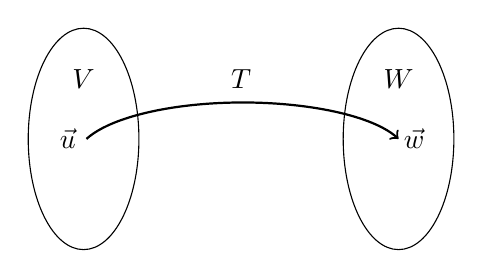
\begin{tikzpicture}
        \draw (2,0) ellipse (20pt and 40pt);
        \draw[] (-2,0) ellipse (20pt and 40pt);
        \draw[<-, thick] (2,0) arc (20:160: 60pt and 20pt);
        \draw (0,1)  node[anchor = north] {$T$};
        \draw (2,1)  node[anchor = north] {$W$}; 
        \draw (-2,1) node[anchor = north] {$V$};
        \draw (-2.2,0) node {$\vec u$};
        \draw (2.2,0) node {$\vec w$};
    \end{tikzpicture}
\end{center}
\subsection{Linear Maps as Vector Space}
Suppose $V$ and $W$ are two linear spaces over $\b F$. $T$ is a function with domain $V$ and codomain $W$. $T$ is called linear iff 
\begin{enumerate}
    \item $T(\vec u_1 + \vec u_2) = T(\vec u_1) + T(\vec u_2)$
    \item $T(\lambda \vec u) = \lambda \cdot T(\vec u)$
\end{enumerate}
$\forall \vec{v}_1, \vec{v}_2 \in V$ and $\forall \vec v_1 \vec v_2 \in V, \forall \lambda\in \b F$.
\begin{example}
    Let $V = \b R^3, W = \b R^4$. Define $T$ as $(x_1, x_2, x_3) \mapsto (x_1,0,0,0)$
\end{example}
\begin{example}
    $T: \c P(x) \to \c P(x)$, where $\displaystyle f(x) \mapsto \int_{10}^x f(x) \ dx$ is a linear map.
\end{example}
\begin{definition}
    $\c L\{V, W\}$ denotes the set of all linear maps from $V$ to $W$. Note that $\c L\{V, W\}$ with $+$ and $\cdot$ becomes a vector space over $\b F$. This requires the additions of functions and multiplications of linear maps by scalars (from $\b F$). Given $T_1, T_2 \in \c L(V,W)$ we define addition as $(T_1 + T_2)(\vec u) := T_1(\vec u) + T_2(\vec u)$, multiplication as $(\lambda T)(\vec u) : = \lambda \cdot T(\vec u)$. 
\end{definition}
\begin{theorem}
    In finite vector space $V,W$, let $\li{\vec u}n$ be a basis for $V$, let $\li{\vec w}m$ be any vectors in $W$. Then there exist a unique linear map $T \in \c L \lb V, W \rb$ such that $T(\vec u_j) = \vec w_j \forall j$.
\end{theorem}
\begin{proof}
    Any vector in $V$ has a unique representation $\alpha_1\vec u_1 + \alpha_2\vec u_2 + \cdots + \alpha_n \vec u_n = \vec u$.  \\ Define $T(u):= \underbrace{\lincomb \alpha {T(\vec u)}n}_{\in W}$ This makes $T$ a linear map from $V$ to $W$. Indeed if $\lambda \in \b F$, then $T(\lambda u) = T(\sum_{j = 1}^n \lambda \alpha_j \vec u_j) = \lambda \sum_{j = 1}^n \alpha_j \vec wj$. Suppose $\tilde T(\vec u_j) = \vec w_j$ for all $j$, then $T = \tilde T$ as a map function by linearity and basis.
\end{proof}
\subsection{Null Space and Range}
\begin{theorem}
    Let $\nul (T):= \lb \vec u \in V : T(\vec u) = 0 \rb$. $\nul (T)$ is a subspace of $V$.
\end{theorem}
\begin{theorem}
    Let $\range (T):= \lb \vec w \in W : T(\vec u) = \vec w \rb$. $\range(T)$ is a subspace of $W$.
\end{theorem}
\begin{proof}
    The proof is trivial and is left as an exercise for the reader.
\end{proof}
\begin{example}
    Let $T: f \to f', V:= \c P(x), W:= \c P(x)$. $\nul(T) = \c P_0(x)$, $\range(T) = \c P_2(x)$. \\
    Let $T: f \to f'', V:= \c P(x), W:= \c P(x)$. $\nul(T) = \c P_1(x)$, $\range(T) = \c P_1(x)$.
\end{example}
\begin{example}
    Find a basis of $\c L (V,W)$ given bases $\lb \li{\vec u}m \rb$ and $\lb \li{\vec w}n \rb$ of $V$ and $W$. \\
    The basis consists of $m \times n$ vectors as follows: 
    \[T_{11} = T(\vec u_1) = \vec w_1, T(\vec u_2) = \vec 0, T(\vec u_3) = \vec 0, \ldots ,T(\vec u_m) = \vec 0\]
    \[T_{12} = T(\vec u_1) = \vec w_2, T(\vec u_2) = \vec 0, T(\vec u_3) = \vec 0, \ldots ,T(\vec u_m) = \vec 0\]
    \[ \cdots \]
    \[T_{mn} = T(\vec u_1) = \vec 0, T(\vec u_2) = \vec 0, T(\vec u_3) = \vec 0, \ldots ,T(\vec u_m) = \vec w_n\]
\end{example}
\begin{example}
    Let $\c U = \lb f : \b R \to \b R : f(x) = f(1-x) \ \forall x \rb$.
    \begin{enumerate}
        \item Show that $\c U$ is a subspace of $f: \b R \to \b R$. 
        
        \item Find a complement.
        \[ \c W  = \lb g : \b R \to \b R : g(x) = -g(1 - x) \ \forall x \rb\]
        
    \end{enumerate}
\end{example}
\begin{proof}
            We can see that the zero function $f(x) = 0$ satisfies the requirement since $0 = 0$ for all  values of $x$. 
            
            Suppose $f(x), g(x) \in \c U$, then we compute \begin{align*}
                (f + g)(x) &= f(x) + g(x) \\
                           &= f(1 - x) + g(1 - x) \\
                           &= (f + g)(1 - x)
            \end{align*}
            Therefore we can see that $\c U$ is closed under addition.
            
            Suppose $f(x) \in \c U, \lambda \in \b R$, then we compute \begin{align*}
                (\lambda \cdot f)(x) &= \lambda \cdot f(x) \\
                                     &= \lambda \cdot f(1 - x) \\
                                     &= (\lambda \cdot f)(1 - x)
            \end{align*}
            Therefore we can see that $\c U$ is closed addition. 
            Hence $\c U$ is a vector space.
        \end{proof}
\begin{proof}
            The proof for subspace is similar to part (i) and is omitted here. \\
            We now want to show that $\c U + \c W  = \mathbb{R}^{\mathbb{R}}$. We can see that for $f(x) \in \mathbb{R}^{\mathbb{R}}$, we can rewrite $f(x)$ as
            \[ f(x) = \frac{f(x) + f(1 - x)}{2} + \frac{f(x) - f(1 - x)}{2}\]
            Clearly $\displaystyle \frac{f(x) + f(1 -x)}{2} \in \c U$ and $\displaystyle \frac{f(x) - f(1 - x)}{2} \in \c W$. For uniqueness, suppose that a nonzero $h(x) \in \c U \cap \c W$, therefore $h(x) = h(1 - x) = -h(1 - x)$, and the only solution is $f(x) = 0$, a contradiction, therefore $\c U \cap \c W = \lb 0 \rb$. Hence $\boxed{{\b R^{\b{R}}} = \c U \oplus \c W}$
        \end{proof}
\begin{theorem}[Rank-Nullity Theorem also known as the Fundamental Theorem of Linear Maps]
    Let $V,M$ be finite dimensional vector spaces, let $T \in \mathcal L(V,W)$. Then
    \[ \dim V = \dim \nul T + \dim \range T\]
\end{theorem}
\begin{proof}
    Let $\li{\vec u}k$ to be the the basis for the basis for $\nul T$. By the linear independent list extension theory, this list can be extended to a basis of $V$. Say $\li{\vec u}k, \li{\vec v}l$ is asujc an extension to a basis of $V$. We can see that $\dim = k + l$. We want to show that $\range T = l$. Consider $\li{T \vec v}l$. We want to show that $\li{T \vec v}l$ is basis for $\range T$. Notice that $\vec v \in V$ can be written as a linear combination of $\lincomb{\alpha}{\vec u}{k} + \lincomb{\beta}{\vec v}{l}$. Then we compute \begin{align*}T\vec v &= \lincomb{\alpha}{T\vec u}{k} + \lincomb{\beta}{T\vec v}{l} \\ &= \lincomb{\beta}{T\vec v}{l} \end{align*} hence $T\vec u \in \spa (\li{T\vec v}{l})$. \\
    Suppose $\lincomb{\beta}{T\vec v}{l} = 0$. Then $\lincomb{\beta}{T\vec v}{l} \in \nul T$. So \[\lincomb{\beta}{\vec v}{l} = \lincomb{\alpha}{\vec u}{k}\] for some $\li{\alpha}{k}$ since $\li{\vec u}k$ form a basis for $\nul T$. \\
    But $\li {\vec v}l, \li{\vec v}k$ form a basis for $V$, all of the coefficient has to be $0$. Therefore $\li{T\vec v}k$ is indeed a basis for $\range T$.
\end{proof}
\begin{example}[Direct consequences of the Theorem]
    Suppose $\dim W < \dim V$ (both finite), and $T \in \c L(V,W)$. Then $T$ cannot be injective.
\end{example}
\begin{proof}
    $T$ is injective implies that $\nul T = \lb \vec 0 \rb$. So $\dim V = 0 + \dim \range T \leq \dim W < \dim V$, a contradiction. 
\end{proof}
\begin{example}[Direct consequences of the Theorem]
    Suppose $\dim W > \dim V$ (both finite), and $T \in \c L(V,W)$. Then $T$  cannot be surjective.
\end{example}
\begin{proof}
    $T$ is surjective implies that $\range T = W$. So $\dim V = \dim \nul T + \dim \range T \geq \dim W > \dim V$, a contradiction. 
\end{proof}
\begin{example}[Fun Question]
    Suppose that $p \in \c P(\b R)$, prove that $\exists q \in \c P(\b R)$ such that $5q'' + 3q' = p$. \\
    \noindent [\textit{This exercise can be done without linear algebra, but it’s more fun to do it using linear algebra.}]
\end{example}
\begin{proof}
    Let $d = \deg p$. Define linear transformation $T: \c P_{d +1}(\b R) \to P_d(\b R)$ as $T: q \to 5q''  +3q'$. We can see that $\dim \nul T  = 1$, by the rank nullity theorem, know that $T$ must be surjective as $\dim \c P_{d+1}(\b R) = \dim \nul T + \dim \range T = 1 + \dim \range \implies \dim \range T = \dim P_d(\b R)$.
\end{proof}
\subsection{Matrix Notation}
\begin{center}
    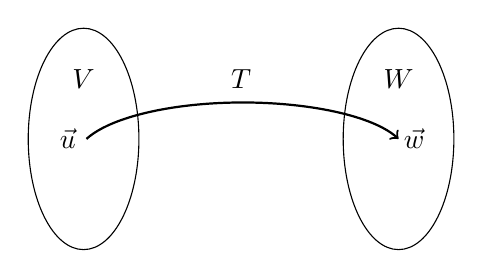
\begin{tikzpicture}
        \draw (2,0) ellipse (20pt and 40pt);
        \draw[] (-2,0) ellipse (20pt and 40pt);
        \draw[<-, thick] (2,0) arc (20:160: 60pt and 20pt);
        \draw (0,1)  node[anchor = north] {$T$};
        \draw (2,1)  node[anchor = north] {$W$}; 
        \draw (-2,1) node[anchor = north] {$V$};
        \draw (-2.2,0) node {$\vec u$};
        \draw (2.2,0) node {$\vec w$};
    \end{tikzpicture}
\end{center}
Recall this diagram, we want to understand $T$ ``correctly". Pick a basis $\li{\vec v}n$ for $V$ and $\li{\vec w}m$ for $W$. We can see that $\dim V = n$ and $\dim W = m$. We can define $T$ as
\[Tv_j = A_{1,j} \vec w_1 + A_{2,j} \vec w_2 + \cdots + A_{m,j} \vec w_m \]
Notice that $A$ has the following form
\[ \begin{array}{cc}
     \vec w_1 \to \\
     \vec w_2 \to \\
     \vdots \\
     \vec w_m \to
\end{array}\bml A_{1,1} & A_{1,2} & \cdots & A_{1,n} \\ 
A_{2,1} & A_{2,2} & \cdots & A_{2,n} \\
\vdots & \vdots & \ddots & \vdots \\ 
A_{m,1} & A_{m,2} & \cdots & A_{m,n} \bmr\]
This is called the matrix representation of $T$.
\begin{example}
    Let $D: V \to W$ be defined as $D := p \to p'$. Let $V:= \spa (1, \cos x, \sin x, \cos 2x, \sin 2x) = W$. We can see that 
    \[\begin{array}{rl}
         1 &\hspace{-0.25cm}\mapsto 0 \\ \cos x &\hspace{-0.25cm}\mapsto -\sin x \\ \sin x &\hspace{-0.25cm}\mapsto \cos x \\ \cos 2x &\hspace{-0.25cm}\mapsto -2 \sin 2x \\ \sin 2x &\hspace{-0.25cm}\mapsto \cos 2x
    \end{array} A = \bml 0 & 0 & 0 & 0 & 0 \\ 
               0 & 0 & -1 & 0 & 0 \\
               0 & 1 & 0 & 0 & 0 \\
               0 & 0 & 0 & 0 & -2 \\
               0 & 0 & 0 & 2 & 0 \bmr\]
\end{example}
\subsection{Matrix Representation} 
Recall that if $T$ is a linear transformation
\begin{center}
    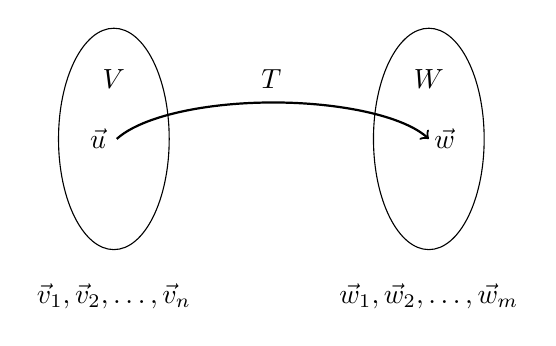
\begin{tikzpicture}
        \draw (2,0) ellipse (20pt and 40pt);
        \draw[] (-2,0) ellipse (20pt and 40pt);
        \draw[<-, thick] (2,0) arc (20:160: 60pt and 20pt);
        \draw (0,1)  node[anchor = north] {$T$};
        \draw (2,1)  node[anchor = north] {$W$}; 
        \draw (-2,1) node[anchor = north] {$V$};
        \draw (-2.2,0) node {$\vec u$};
        \draw (2.2,0) node {$\vec w$};
        \draw (-2, -2) node {$\li{\vec v}n$};
        \draw (2, -2) node {$\li{\vec w}m$};
    \end{tikzpicture}
\end{center}
\[ T\vec v_u = \sum_{k = 1}^{m} A_{i,k} \vec w_k \]
Note that Matrix $A = \left[ A_{i,k} \right]$ has $m$ rows $n$ columns.
\[\left[ \begin{array}{cccc} A_{1,1} & A_{1,2} & \cdots & A_{1,n} \\
        A_{2,1} & A_{2,2} & \cdots & A_{2,n} \\
        \vdots & \vdots & \ddots & \vdots  \\
        A_{m,1} & A_{m,2} & \cdots & A_{m,n} \\
        \end{array} \right]\]
Suppose $v = \lincomb{c}{\vec v}{n}, T\vec v = \lincomb{c}{T\vec v}{n}$.
\[T\vec v =  c_1 \sum_{i=1}^m A_{i,1} \vec w_1  +  c_2 \sum_{i=1}^m A_{i,2} \vec w_2 + \cdots + c_n \sum_{i=1}^m A_{i,n} \vec w_n = \sum_{i = 1}^m \left( \sum_{i = 1}^n A_{i,j} c_j \right) \vec w_j \]
Notice that the operation is the equivalent as the matrix-vector multiplication.
\begin{center}
    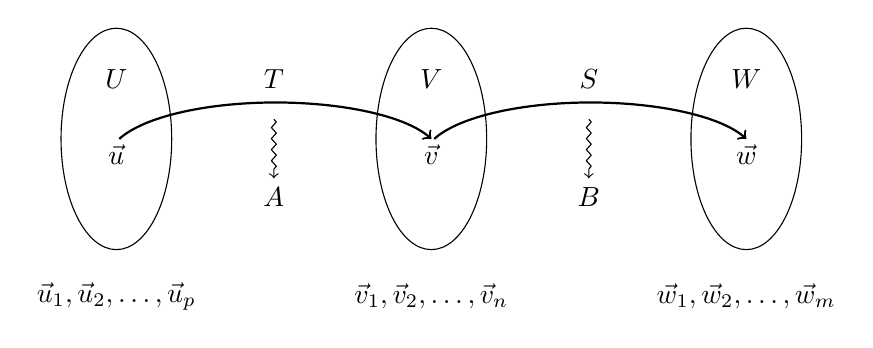
\begin{tikzpicture}
        \draw (2,0) ellipse (20pt and 40pt);
        \draw (-2,0) ellipse (20pt and 40pt);
        \draw (6,0) ellipse (20pt and 40pt);
        \draw[<-, thick] (2,0) arc (20:160: 60pt and 20pt);
        \draw[<-, thick] (6,0) arc (20:160: 60pt and 20pt);
        \draw (0,1)  node[anchor = north] {$T$};
        
        \draw (2,1)  node[anchor = north] {$V$}; 
        \draw (-2,1) node[anchor = north] {$U$};
        \draw (6,1) node[anchor = north] {$W$};
        \draw (4,1) node[anchor = north] {$S$};
        \draw[->, line join=round, decorate, decoration={
    zigzag, segment length=4,
    amplitude=.9,post=lineto,
    post length=2pt }] (0,0.25) -- (0,-0.5);
        \draw[->, line join=round, decorate, decoration={
    zigzag, segment length=4,
    amplitude=.9,post=lineto,
    post length=2pt }] (4,0.25) -- (4,-0.5);
        \draw (0,-0.5) node[anchor = north] {$A$};
        \draw (4,-0.5) node[anchor = north] {$B$};

        \draw (-2,-0.2) node {$\vec u$};
        \draw (2, -0.2) node {$\vec v$};
        \draw (6, -0.2) node {$\vec w$};
        \draw (-2, -2) node {$\li{\vec u}p$};
        \draw (2, -2) node {$\li{\vec v}n$};
        \draw (6, -2) node {$\li{\vec w}m$};
    \end{tikzpicture}
\end{center}
\[ ST\vec u_k = S(T\vec u_k) = S \left( \sum_{j=1}^n A_{j,k}\vec v_j \right) = \sum_{j = 1}^{n} A_{j,k} \left(S\vec v_j\right) = \sum_{j = 1}^n A_{j,k} \sum_{i = 1}^{m} B_{i,j} \vec w_i = \sum_{i = 1}^m \left( \sum_{j = 1}^n B_{i,j}A_{j,k} \right) \vec w_i\]
Use name $\c M(S) := B$, $\c M(T) := A$, $\c M(ST) = BA = \c M(S) \cdot \c M(T)$.
So matrix representation multiply as matrices to produce a composition map or product.
\begin{remark}[Book Keeping]
    $A_{\ast, j}$ denotes the $j$th column of $A$. \\
    $A_{i, \ast}$ denotes the $i$th row of $A$.
\end{remark}
Notice that $\c M$ is a linear map, $\c L (V,W) \xrightarrow{\c M} \b F^{m,n}$. 
\begin{proposition}
    $\c M$ is a linear map.
\end{proposition}

\begin{proposition}
    $\b F^{m,n}$ has a basis.
\end{proposition}
\begin{proof}
    Consider $E_{i,j}$, the matrix consists of all zeros with the exception of $1$ in position $(i,j)$. This can be done for all $i = 1, 2, \ldots, m$, $j  =1,2, \ldots, n$. Also notice that $\dim \b F^{m,n} = m \cdot n$
\end{proof}

\subsection{Invertibility and Isomorphism}
\begin{center}
    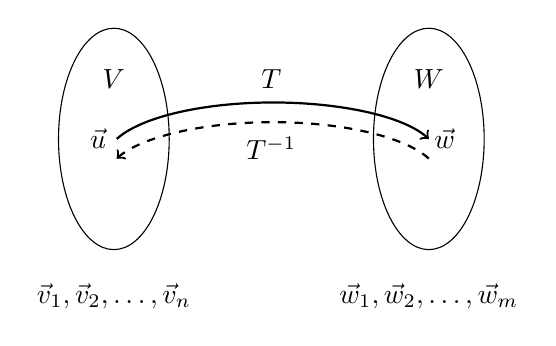
\begin{tikzpicture}
        \draw (2,0) ellipse (20pt and 40pt);
        \draw[] (-2,0) ellipse (20pt and 40pt);
        \draw[<-, thick] (2,0) arc (20:160: 60pt and 20pt);
        \draw[->, thick,style = dashed] (2,-0.25) arc (20:160: 60pt and 20pt);
        \draw (0,1)  node[anchor = north] {$T$};
        \draw (0,0.15)  node[anchor = north] {$T^{-1}$};
        \draw (2,1)  node[anchor = north] {$W$}; 
        \draw (-2,1) node[anchor = north] {$V$};
        \draw (-2.2,0) node {$\vec u$};
        \draw (2.2,0) node {$\vec w$};
        \draw (-2, -2) node {$\li{\vec v}n$};
        \draw (2, -2) node {$\li{\vec w}m$};
    \end{tikzpicture}
\end{center}
\begin{definition}
    $T \in \c L(V,W)$ is invertible provided that there exists a mapping $T^{-1}$ from $W$ to $V$ (not necessarily linear) such that \[ T^{-1} \circ T = \b I_V\]
    \[ T \circ T^{-1} = \b I_W\]
    Where $\b I_{V}, \b I_W$ is the identity map on $V$ and $W$.
\end{definition}
\begin{theorem}
    $T$ is invertible if and only if $T$ is both injective and surjective.
\end{theorem}
\begin{proof}
    Suppose $T$ is invertible, then $T(T^{-1} \vec w) = \vec w \ \forall \vec w \in W$, so $\range T = W$. Also we know that $T^{-1}(T \vec v) = \vec v$. Suppose $T\vec v_1 =T\vec v_2$, apply the left inverse and we have $T^{-1} (T\vec v_1) = T^{-1} (T\vec v_2) \implies \vec v_1 = \vec v_2$. Hence $T$ is injective. Therefore $T$ is bijective. \\
    Now suppose $T$ is bijective. We want to construct $T^{-1}$
    \begin{center}
    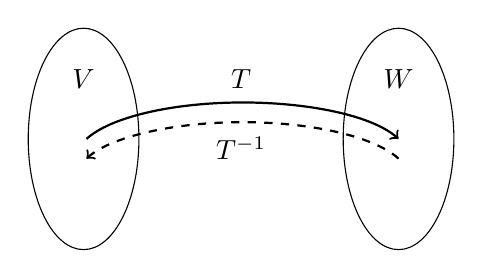
\begin{tikzpicture}
        \draw (2,0) ellipse (20pt and 40pt);
        \draw[] (-2,0) ellipse (20pt and 40pt);
        \draw[<-, thick] (2,0) arc (20:160: 60pt and 20pt);
        \draw[->, thick,style = dashed] (2,-0.25) arc (20:160: 60pt and 20pt);
        \draw (0,1)  node[anchor = north] {$T$};
        \draw (0,0.15)  node[anchor = north] {$T^{-1}$};
        \draw (2,1)  node[anchor = north] {$W$}; 
        \draw (-2,1) node[anchor = north] {$V$};
    \end{tikzpicture}
\end{center}
We need to take $\vec w \in W$, there is a $\vec v \in V$ such that $T\vec v = \vec w$ and such $\vec v$ is unique since $T$ is injective. We declare $T^{-1}\vec w$ to be $\vec v$. So $T^{-1} \circ T = \b I_{V}$. We compute \[ (T \circ T^{-1}) \vec w = T(T^{-1} \vec w) = T\vec v = \vec w \ \forall  \vec w \in W\] So $T \circ T^{-1} = \b I_W$ 
\end{proof}
\begin{definition}
    If $V,W$ are vector spaces, such that there exists a invertible linear map $T \in \c L(V,W)$ then $V, W$ are isomorphic.
\end{definition}
\begin{remark}
    Before we proceed, we want to check that $T^{-1}$ is a linear map when $T \in \c L(V,W)$ and $T^{-1}$ exists.
\end{remark}
\begin{proof}
    Take $\vec w_1,\vec w_2 \in W, \lambda \in \b F$. We compute
    $T^{-1} (\lambda \vec w_1 + \vec w_2)$. We know that $\vec w_1 = T\vec v_1$ and $\vec w_2 = T\vec v_2$. Then we know that $T(\lambda \vec v_1  + \lambda \vec v_2) = \lambda T\vec v_1 + T\vec v_2 = \lambda\vec  w_1 +\vec  w_2$. Subsitute this into $T^{-1}$ and we get
    \[ T^{-1} (\lambda \vec w_1 + \vec w_2) = T^{-1} \circ T (\lambda \vec v_1 + \vec v_2) = \b I (\lambda \vec v_1 + \vec v_2) = \lambda \vec v_1 + \vec v_2 = \lambda T^{-1} \vec w_1 + T^{-1} \vec w_2\] Hence $T^{-1}$ is linear.
\end{proof}
\begin{corollary}
    $\c M$ is actually a bijection between $\c L(V,W)$ and $\b F^{m,n}$, therefore $\c L(V,W)$ is isomorphic to $\b F^{m,n}$.
\end{corollary}
\begin{theorem}
    Suppose $T \in \c L(V,W)$ is linear and invertible, and let $\li {\vec v}m$ be a basis for $V$. Then $\li{T\vec v}n$ is a basis for $W$.
\end{theorem}
\begin{proof}
    Suppose $\lincomb{\alpha}{T\vec v}{n} = 0$. Then $T(\lincomb{\alpha}{\vec v}{n}) = 0$. Since $T$ is injective, this implies $\lincomb{\alpha}{\vec v}{n} = 0$. Therefore $\alpha_1 = \alpha_2 = \cdots = \alpha_n = 0$ since $\li{\vec v}n$ is a basis. Take $\vec w \in W$, then there exists a unique $\vec v \in V$ such that $T\vec v = \vec w$, and $\vec v = \lincomb{\alpha}{\vec v}{n}$ for some $\li \alpha n$, so $T\vec v = \vec w = \lincomb{\alpha}{T\vec v}{n}$, hence span. 
\end{proof}
\begin{corollary}
    $\dim$ is invariant under isomorphism.
\end{corollary}
\subsubsection*{Linear Operators}
We are dealing with a specific case where $\c L(V,W)$ is replaced by $\c L(V,V)$.
\begin{center}
    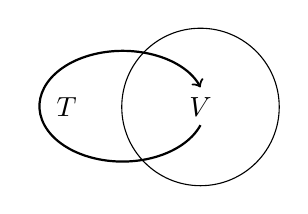
\begin{tikzpicture}
        \draw[<-, thick] (0,0.25) arc (20:340: 30pt and 20pt);
        \draw (0,0) circle(1);
        \draw (0,0) node{$V$};
        \draw (-1.7,0) node{$T$};
    \end{tikzpicture}
\end{center}
Recall that $\dim V = \dim \nul T + \dim \range T$. This gives a better test for invertablity if $W  = V$. 
\begin{theorem}
    Let $T \in \c L(V,V)$. If $V$ is finite dimensional vector space, then the following are equivalent: 
    \begin{enumerate}[label = (\alph*)]
        \item $T$ is injective.
        \item $T$ is surjective.
        \item $T$ is invertible.
    \end{enumerate}
\end{theorem}
\begin{proof} $ $ \\
    (a) $\implies$ (c). Trivial by definition. \\
    (b) $\implies$ (c). Suppose $T$ is injective $\xRightarrow[T \text{ being linear}]{} \nul T = \lb 0 \rb \iff \dim \nul T = 0$. Therefore 
    \[ \dim V = \dim \nul T = \dim \range T = 0\] So $\dim V = \dim \range T$, hence $\range T = V$, so $T$ is surjective. \\
    (c) $\implies$ (a).  \[\dim V = \dim \nul T + \dim \range T = \dim \nul T + \dim V \implies \dim \nul T  = 0 \implies \nul T = \lb \vec 0 \rb\] So $T$ is injective. $T$ is already known to be surjective, so $T$ is bijective, or $T$ is invertable.
\end{proof}
\begin{example}
    The theorem does not hold for infinite dimension vector spaces, for example: \\ 
    The differentiation map $T : f(x) \mapsto f'(x)$ is surjective but not invertible over $\c P(\b R)$.  From calculus we know that for every $f(x) \in \c P(\b R)$, there exists $g(x) \in \c P(\b R)$ such that $g'(x) = f(x)$, however, we can see that $\nul T \neq \lb 0 \rb$ as $1 \in
    \nul T$. Hence $T$ is not injective. \\
    The integration map $\displaystyle T: f(x) \mapsto \int_0^x f(t) dt$ is injective but not invertible over $\c P(\b R)$. We can see that $\nul T = \lb 0 \rb$, hence $T$ is injective, however, $1 \not\in \range T$.
\end{example}
\subsection{Duality}
\begin{definition}
    Given a vector space $V$, we define its dual space as $V' = \c L(V,\b F)$. 
\end{definition}
\begin{remark}
    Objects in $\c L(V,\b F)$ are also called linear functional.
\end{remark}
\begin{example}
    Linear Functional on $\b R^3$: $(x_1, x_2, x_3) \mapsto \alpha_1 x_1 + \alpha_2 x_2 + \alpha_3 x_3 \ \forall \alpha_1, \alpha_2, \alpha_3 \in \b R$.
\end{example}
\begin{definition}
    Suppose $\li{\vec v}n$ is a basis of $V$. The list of linear functionals $\li \varphi n \in  V'$ such that \[\varphi_i(\vec v_j) = \left\{ \begin{array}{cc}
         1 \text{ if } i = j \\
         0 \text{ if } i \neq j
    \end{array} \right.\] We claim that $\li\varphi n$ is the dual basis of $V'$.
\end{definition}
\begin{lemma}
    A dual basis is a basis of $V'$.
\end{lemma}
\begin{proof}
    Suppose there exists $\li \alpha n$ such that 
    \[ \lincomb{\alpha}{\varphi}{n} = 0\]
    We compute for $v_1$
    \[ (\lincomb{\alpha}{\varphi}{n})(n) = \alpha_1 \cdot 1 + 0 \implies \alpha_1 = 0\]
    Similarly, if we plug in an arbitrary $v_j$
    \[ (\lincomb{\alpha}{\varphi}{n})\vec v_j) \implies v_j = 0\]
    This shows that $\li \varphi n$ is linear independent, and the count is $n$. So $\li \varphi n$ form a basis for $V'$.
\end{proof}
\subsubsection*{Dual Maps}
\begin{center}
    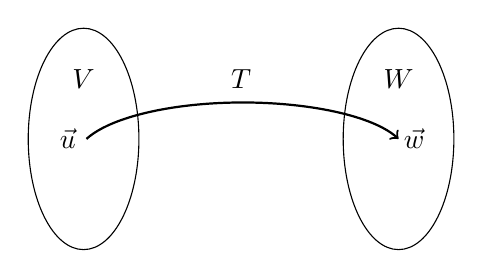
\begin{tikzpicture}
        \draw (2,0) ellipse (20pt and 40pt);
        \draw[] (-2,0) ellipse (20pt and 40pt);
        \draw[<-, thick] (2,0) arc (20:160: 60pt and 20pt);
        \draw (0,1)  node[anchor = north] {$T$};
        \draw (2,1)  node[anchor = north] {$W$}; 
        \draw (-2,1) node[anchor = north] {$V$};
        \draw (-2.2,0) node {$\vec u$};
        \draw (2.2,0) node {$\vec w$};
    \end{tikzpicture}
\end{center}
\begin{center}
    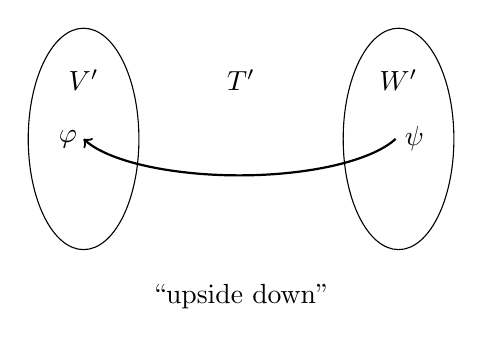
\begin{tikzpicture}
        \draw (2,0) ellipse (20pt and 40pt);
        \draw[] (-2,0) ellipse (20pt and 40pt);
        \draw[<-, thick] (-2,0) arc (200:340: 60pt and 20pt);
        \draw (0,1)  node[anchor = north] {$T'$};
        \draw (2,1)  node[anchor = north] {$W'$}; 
        \draw (-2,1) node[anchor = north] {$V'$};
        \draw (-2.2,0) node {$\varphi$};
        \draw (2.2,0) node {$\psi$};
        \draw (0, -2) node {``upside down"};
    \end{tikzpicture}
\end{center}
\begin{definition}
    Given $T \in \c L(V,W)$, we define $T' : \varphi \mapsto \varphi \circ T$. $ \phi \in W'$ i.e. $\varphi \in \c L(W, \b F)$. Notice that $\varphi \circ T \in \c L(V, \b F)$.
\end{definition}
\begin{example}
    Define $V, W, \varphi, T$ as $\varphi : f \mapsto \int_0^1 f(t) dt, V = \c P_3(\b R), W = \c P_2(\b R), T : f \mapsto f'$. What is $\varphi \circ T$? 
    \[ (\varphi \circ T)(f) = \varphi(T(f)) = \varphi (f') = \int_0^1 f'(t)dt = f(1) - f(0)\]
\end{example}
\begin{remark}[Algebraic Property of dual maps] $ $
    \vspace{-0.5cm}
    \begin{enumerate}
        \item $(S + T)'  = S' + T'$
        \begin{proof}
            For any $S,T \in \c L(V,W), S', T' \in \c L(W',V')$ , we compute 
            \[(S + T)'(\varphi) = \varphi \circ (S + T) = \varphi \circ S + \varphi \circ T = S'(\varphi) + T'(\varphi)\]
        \end{proof}
        \item $(\lambda S)' = \lambda S'$
        \begin{proof}
            \[ (\lambda S)'(\varphi) = \varphi \circ (\lambda S) = \lambda (\varphi \circ S) = \lambda \cdot S'(\varphi)\]
        \end{proof}
        \item $(ST)'  = T' S'$
        \begin{proof}
            Sanity check: $S \in \c L(V,W), T \in \c L(U,V)$
            \[ (ST)' : \varphi \mapsto \varphi 
            \circ (ST) = (\varphi \circ S) \circ T = T'(\varphi \circ S) = T'(S'(\varphi)) = T' \circ S'\]
        \end{proof}
    \end{enumerate}
\end{remark}
\begin{definition}[Annihilators]
    Let a set $S$ to be a subset of a vector space $V$. We can define $S^0$ as 
    \[ S^0 := \lb \varphi \in V' : \varphi (v) = 0 \ \forall \vec v \in S \rb\]
\end{definition}
\begin{example}
    Consider $\b R^3$, let $S := \lb (1,0,0), (1,1,0) \rb$. We know that any $\varphi \in \b R^3$ will have the form of $(x_1,x_2,x_3) \mapsto a_1x_1 + a_2x_2 + a_3x_3$ for some constant $a_1,a_2,a_3$. Plug in $(1,0,0)$ and $(1,1,0)$ and we get 
    \[ a_1 \cdot 1 + a_2 \cdot 0 + a_3 \cdot 0 = 0 \implies a_1 = 0\]
    \[ a_1 \cdot 1 + a_2 \cdot 1 + a_3 \cdot 0 = 0 \implies a_2 = 0\]
    We can see that $S^{0} = \lb \varphi(x_1, x_2, x_3) = a_3 x_3 \text{ for some } a_3 \in \b R \rb$ and forms a subspace for $\b R^{3}$'.
\end{example}
\begin{lemma}
    Regardless of the nature of $S$, $S^0$ is always a subspace.
\end{lemma}
\newpage
\begin{proof}
    \begin{enumerate}
        \item The zero functional is clearly in $S^0$.
        \item Suppose $\varphi \in S^0$, take $\lambda \in \b F$, then $(\lambda \varphi)(\vec v) = \lambda \cdot \varphi(\vec v) = 0$ for all $\vec v \in S$. So $\lambda \varphi \in S$.
        \item Suppose $\varphi, \psi \in S^0$, then $(\varphi + \psi)(\vec v) = \varphi(\vec v) + \psi(\vec v) = 0$ for all $\vec v \in S$. Therefore $\varphi + \psi \in S^0$.
    \end{enumerate}
\end{proof}
\begin{theorem}
    Suppose $S = U$, where $U$ is a subspace of $V$, then 
    \[ \dim U + \dim U^0 = \dim V\]
\end{theorem}
\begin{proof}
    Consider the inclusion map: \[i : U \to V : \vec u \to \vec u \ \forall \vec u \in U\] 
    Take  a look at the dual of $U$: $i' \in \c L(V', U')$. Apply Rank-Nullity to the dual map and we can see that $\dim V' = \dim \nul i' + \dim \range i'$. We also know that \[\nul i' = \lb \varphi \in V' : \varphi \circ i = 0 \rb\] Notice that $\varphi \circ i = 0$ as a functional implies \[(\varphi \circ i) (\vec u) = 0 \implies \varphi(i(\vec u)) = 0 \implies \varphi(\vec u) = 0 \ \forall \vec u \in U \]
    Therefore we can see that $\range i' = \lb \varphi \circ i : \varphi \in V' \rb = U'$ since any linear functional on $U$ extends to $V$. I have a clever proof for this but it does not fit in the margin of the page and is left as an exercise for the reader. 
\end{proof}
\begin{theorem}
    Let $V,W$ be finite dimensional vector space and let $T \in \c L(V,W)$. Then 
    \begin{enumerate}[label = (\alph*)]
        \item $\nul T' = (\range T)^0$
        \item $\dim \nul T' = \dim \nul T + \dim W - \dim V$
    \end{enumerate}
\end{theorem}
\begin{proof} $ $
    \begin{enumerate}[label = (\alph*)]
        \item $\varphi \in \nul T' \iff \varphi \circ T = 0 \iff (\varphi \circ T)(\vec v) = 0 \ \forall \vec v \in V \iff \varphi(T\vec v) = 0 \ \forall \vec v \in V \\ \iff \varphi \in (\range T)^0$
        \item $\dim \nul T' = \dim (\range T)^0 = \dim W - \dim \range T = \dim W - (\dim V - \dim \nul T) = \dim W - \dim V + \dim \nul T$
    \end{enumerate}
\end{proof}
\begin{corollary}
    $T'$ is injective if and only if $T$ is surjective.
\end{corollary}
\begin{theorem}
    Suppose $V$ and $W$ are finite dimensional and $T \in \c L(V,W)$, then 
    \begin{enumerate}[label = (\alph*)]
        \item $\dim \range T' = \dim \range T$
        \item $\range T' = (\nul T)^0$
    \end{enumerate}
\end{theorem}
\begin{proof} $ $
    \begin{enumerate}[label = (\alph*)]
        \item $\dim \range T' = \dim W' - \dim \nul T' = \dim W - (\dim W - \dim V + \dim \nul T) = \dim V - \dim \nul T = \dim \range T$
        \item $\psi \in \range T' \iff \exists \varphi : \varphi \circ T = \psi \iff \varphi \circ T(\vec v) = \psi(\vec v) \ \forall \vec v \in V \iff \varphi(T\vec v) = \psi(\vec v) \forall \vec v \in V$. \\ So $T\vec v = 0 \implies \psi(\vec v) = 0$. This shows $\range T' \subseteq (\nul T)^0$. But $\dim \range T' = \dim \range T = \dim V - \dim \nul T = \dim (\nul T)^0$. Hence $\range T = \nul T$.
    \end{enumerate}
\end{proof}
\subsubsection{Matrix Representation of the dual map}
Recall that
\begin{center}
    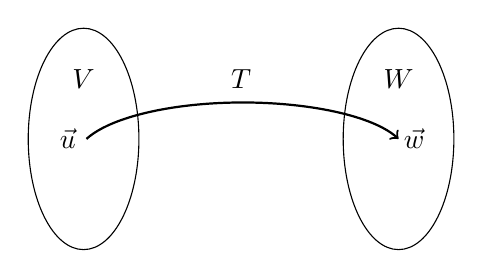
\begin{tikzpicture}
        \draw (2,0) ellipse (20pt and 40pt);
        \draw[] (-2,0) ellipse (20pt and 40pt);
        \draw[<-, thick] (2,0) arc (20:160: 60pt and 20pt);
        \draw (0,1)  node[anchor = north] {$T$};
        \draw (2,1)  node[anchor = north] {$W$}; 
        \draw (-2,1) node[anchor = north] {$V$};
        \draw (-2.2,0) node {$\vec u$};
        \draw (2.2,0) node {$\vec w$};
    \end{tikzpicture}
\end{center}
\begin{center}
    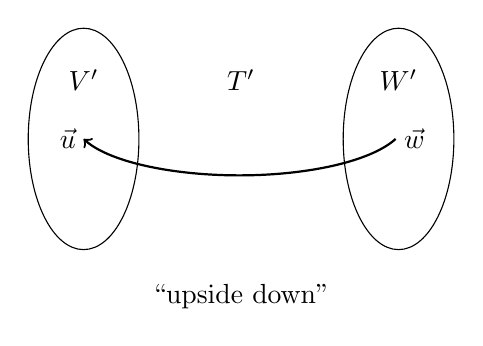
\begin{tikzpicture}
        \draw (2,0) ellipse (20pt and 40pt);
        \draw[] (-2,0) ellipse (20pt and 40pt);
        \draw[<-, thick] (-2,0) arc (200:340: 60pt and 20pt);
        \draw (0,1)  node[anchor = north] {$T'$};
        \draw (2,1)  node[anchor = north] {$W'$}; 
        \draw (-2,1) node[anchor = north] {$V'$};
        \draw (-2.2,0) node {$\vec u$};
        \draw (2.2,0) node {$\vec w$};
        \draw (0, -2) node {``upside down"};
    \end{tikzpicture}
\end{center}
We also recall that $T' : \varphi \mapsto \varphi \circ T$.
\newpage
\begin{question}
    How do we get $\c M(T')$ given $\c M(T)$?
\end{question}
\begin{answer}
For $\c M(T)$, we need $2$ bases $\li {\vec v}n$ for $V$ and $\li {\vec w}m$ for $W$. \\
    Take $\li \varphi n$, a dual basis to $\li {\vec v}n$, it is a basis for $V'$. \\
    Tale $\li \psi m$, a dual basis to $\li {\vec w}m$, it is a basis for $W'$. \\
    Given $\c M(T)$, we want to construct / understand $\c M(T')$with regard to the basis $\li \psi m$ of $W'$ and $\li \varphi n$ of $V'$. \\
    We know $\c M(T)$ has $m$ rows $n$ columns, and $\c M(T')$ has $n$ rows and $m$ columns. \\Suppose $\c M(T) = A, \c M(T') = C$, we then know 
    \[ T\vec v_j = \sum_{i = 1}^m A_{i,j} \vec w_i \ \forall j = 1,2, \ldots, n, T'\psi_l = \sum_{l = 1}^n C_{l,k} \varphi_{l} \ \forall l =  1,2,\ldots, m\]
    \[ T' \psi_k = \psi_k \circ T \implies (\psi_k \circ T )(\vec v_j) = \psi_k(T\vec v_j) = \psi_k \left( \sum_{i=1}^m A_{i,j} \vec w_j \right) = \sum_{i = 1}^m A_{i,j} \psi_k(\vec w_i) = \sum_{i = 1}^m A_{i,j} \delta_{ki} = A_{k,j}\]
    \[(T'\psi_k)(\vec v_j) = \left( \sum_{l = 1}^{n} C_{l,k} \varphi_l \right) (\vec v_j) = \sum_{l = 1}^{n} C_{l,k} \varphi(\vec v_j) = \sum_{l = 1}^{n} C_{l,k} \delta_{l,j} = C_{j,k} \]
    Notice that $A_{k,j} = C_{j,k} \ \forall j,k$.
\end{answer}
\begin{conjecture}
    So we obtained that 
    \[ M(T') = M(T)^{T}\]
    provided that the basis of $V'$ and $W'$ are chosen to be the dual to the bases of $V$ and $W$, respectively.
\end{conjecture}
\begin{example}
    Let $T: p \mapsto p'$ for $V = \c P_3(\b R)$ with basis $1,x,x^2, X^3$, and $W = \c P_2(\b R)$ with $1,x,x^2$. \\
    We can see that the dual basis for $1,x,x^2, x^3$ is \[\varphi_0 : p \mapsto p(0), \varphi_1 : p \mapsto p'(0), \varphi_2: p \mapsto \frac{p''(0)}{2}, \varphi_3 : p \mapsto \frac{p'''(0)}{3!}\]
    Dual basis for $1,x,x^2$ is 
    \[\psi_0 : p \mapsto p(0), \psi_1 : p \mapsto p'(0), \psi_2: p \mapsto \frac{p''(0)}{2}, 
    \]
    Notice that \[\c M(T) = \bml 0 & 1 & 0 & 0 \\ 0 & 0 & 2 & 0 \\ 0 & 0 & 0 & 3\ \bmr \text{ and } \c M(T') = \bml 0 & 0 & 0 \\ 1 & 0 & 0 \\ 0 & 2 & 0 \\ 0 & 0 & 3 \bmr\]
\end{example} \vfill
\section{Polynomials}
Recall we call consider polynomials over $\b C$ or $\b R$.
\begin{theorem}
    For any $z_1, z_2 \in \b C$, we define $|z|  = \sqrt{a^2 + b^2}$, we know that 
    \begin{enumerate}
        \item $|z_1 \cdot z_2| = |z_1| \cdot |z_2|$
        \item $|z_1 \cdot z_2| \leq |z_1| + |z_2|$
    \end{enumerate}
\end{theorem}
\begin{proof}
Left as an execise.
\end{proof}
\subsection{Axler's Recap on Polynomial}
\begin{theorem}
    Suppose $p(x) \in \c P(\b F)$, is identically zero. Then all of its coefficient must be $0$. 
\end{theorem}
\begin{proof}
    If $p(x) = a_0 + a_1x + \cdots + a_nx^n$, then $a_j = \frac{p^{(j0}(0)}{j!}$, If $p(x) \equiv 0$, then $p^{(j)}(x) = 0$, so $a_j = \frac{0}{j!} = 0 \forall j$
\end{proof}
\begin{corollary}
    Suppose $p(x) \equiv q(x)$ for $p,q \in \c P(\b F)$, then all coefficients of $p$ are the same as all coefficients of $q$.
\end{corollary}
\subsection{Zero of polynomials and their algebraic manifestations}
\begin{algorithm}[Euclidean Algorithm for polynomials]
 Given $p(x), s(x)$, without the loss of generality, $\deg p(x) > \deg s(x)$, otherwise it's boring; we can always find $q(x), r(x)$ such that $p(x) = s(x)q(x) + r(x)$, where $\deg r(x) < \deg s(x)$.
\end{algorithm}
\begin{corollary}
    $p(a) \iff p(x) = (x - a)q(x)$ for some $a \in \b F$.
\end{corollary}
\begin{proof}
    If $p(a) = (x-a)q(x)$, then $p(a) = 0 \cdot q(a) = 0$. \\
    Conversely, suppose $p(a) = 0$, by division algorithm we have $p(x) = (x - a)q(x) + r(x)$, where $\deg r \leq \deg (x-a)$, therefore $r(x) = c$ for some $c \in \b F$. Plug in $a$ and we get $(a - a)q(a) + c = 0 \implies 0 + c = 0 \implies c = 0$. Therefore $p(x) = (r-a)q(x)$.
\end{proof}
\begin{theorem}
    Let $p(x)$ be a nonzero polynomial with coefficients in $\b F$ have degree $n$. Then $p$ has at most $n$ zeros in $\b F$.
\end{theorem}

\begin{proof} $ $ \\
    \textit{Base case:} $\deg p = 1$, i.e. $p(x) = a_1x + a_0$ for some $a_1 \in \b F^\times, a_0 \in \b F$. Then $p\left(\frac{-b}{a}\right) = 0$, so $p$ has exactly one zero. \\
    \textit{Inductive Hypothesis:} Suppose the statement is true for all polynomials for all polynomials of degree less than $m$. \\
    \textit{Inductive Step:} Take $p(x)$ to be a degree $m$ polynomial. If $p$ has no zeros in $\b F$, we are done. If $p$ has a zero, by corollary we have $p(x) = (x - a)q(x)$, where $\deg q = m - 1$. So the inductive hypothesis applies and $q$ at most $n-1$ distinct zeros in $\b F$.
\end{proof}
\begin{theorem}[Fundamental Theorem of Algebra]
    Every nonconstant polynomial with complex coefficients has a zero.
\end{theorem}
\begin{proof}[Proof with ``Black Box" from Complex Analysis] $ $ \\
    Assume $\deg p \geq 1$. Assume that $p(a) \neq 0 \ \forall a \in \b C$. Consider the function $\frac{1}{p(x)}$ is well-defined $\forall x \in \b C$ and is analytic in $\b C$, more over $\lim_{|z| \to \infty} \frac{1}{p(z)} = 0$. We know that 
    \begin{align*}
        p(x) &= a_0 + a_1 x + \cdots + a_n x^n \\
        &= x^n \left( \frac{a_0}{x^n} + \frac{a_1}{x^{n-1}} + \cdots + a_n\right) \\
        \frac{1}{p(x)} &= \frac{1}{x^n \left( \frac{a_0}{x^n} + \frac{a_1}{x^{n-1}} + \cdots + a_n\right)} 
    \end{align*}
    As $\displaystyle |x| \to \infty, \displaystyle \frac{1}{x^n} \to 0$. Since $\displaystyle \left|\frac{1}{x^n}\right| = \frac{1}{|x|^n} \to 0$. But $\displaystyle \frac{a_0}{x^n} + \frac{a_1}{x^{n-1}} + \cdots + a_n \to a_n \neq 0$. Hence $\displaystyle \frac{1}{p(x)} \to 0$ as $|x| \to -\infty$. \\
    By Louisville's theorem, any analytic function with this property has to be constant. But $\frac{1}{p(x)}$ is non-constant, so $p$ must have at least $1$ zero in $\b C$.
\end{proof}
\begin{corollary}
    Any polynomial $p(x)$ with coefficients in $\b C$ factors as follows 
    \[ p(x) = c(x - a_1)(x - a_2) \cdots (x - a_m), c \neq 0\]
\end{corollary}
\begin{proof}
    By Induction it's clear for degree $1$ and if $\deg p = m$ then factor $p(x) = (x - a)q(x)$ and repeat the process for $q$.
\end{proof}
\begin{question}
    What happens over $\b R$?
\end{question}
\begin{theorem}
    If $p(x)$ has coefficient in $\b R$, and $c \in \b C$ is a zero of $p$, then $\bar c$ is also a zero of $p$.
\end{theorem}
\begin{proof}
    $p(c) = 0$ means \[a_0 + a_1 c + a_2 c^2 + \cdots + a_nc^n = 0\] We then can see \begin{align*}
        \bar{a_0} + \bar{a_1 c} + \bar{a_2 c^2} + \cdots + \bar{a_n c^n} &= \bar 0 = 0 \\
        \bar{a_0} + \bar{a_1} \bar{c} + \bar{a_2} \bar{c^2} + \cdots + \bar{a_n} \bar{c^n} & = 0 \\
        a_0 + a_1 \bar c + a_2 \bar{c^2} + \cdots + a_n \bar{c^n} &= 0
    \end{align*}
    Hence $p(\bar c) = 0$ as well.
\end{proof}
So over $\b C$, a polynomial with real coefficient factors as follows
\[ p(x) = (x - a_1)(x - a_2)\cdots(x - a_n)(x - \lambda_1)(x - \bar{\lambda_1})(x - \lambda_2)(x - \bar{\lambda_2}) \cdots (x - \lambda_m)(x - \bar{\lambda_m})\]
For some $c \in \b R, \li an \in \b R, \li \lambda m \in \b C$. \\
To translate this into a factorization over $\b R$, we can see that $x^2 - (\lambda + \bar \lambda) + |\lambda|^2$. These are quadratic with $\Delta < 0$. Indeed, 
\[ (\lambda + \bar \lambda)^2 - 4 |\lambda|^2 = \lambda ^2 - 2 |\lambda |^2 + {\bar \lambda}^2 = 2 \text{Re} \lambda^2 - 2 |\lambda|^2 \]
Notice that $\text{Re} \lambda^2 \leq |\lambda|^2$ and $\text{Re} \lambda^2 = |\lambda|^2$ iff $\lambda \in \b R$, therefore $\Delta < 0$.
\begin{question}
    Why do we study polynomials?
\end{question}
\begin{answer} $ $
\begin{enumerate}
    \item We will form polynomials in linear operators
    \item We will associate special polynomials with linear operators.
\end{enumerate}
\end{answer}
\begin{remark}
An operator has he same co-domain as its domain.
\end{remark}

 \vfill
\section{Eigenvalues, Eigenvectors, and
Invariant Subspaces}
\subsection{Invariant Subspaces}
\begin{definition}
    Let $T \in \c L(V,V)$ on a vector space $V \neq \lb 0 \rb$. A subspace $U \subseteq V$ is called an invariant subspace is invariant under $T$ if $Tu \in U \ \forall u \in U$.
\end{definition}
\begin{example}
    For any $T \in \c L(V,V)$, the following subspaces are invariant:
    \begin{enumerate}
        \item $\lb 0 \rb$
        \item $V$
        \item $\nul T = \lb v \in V : Tv = 0 \rb$ \\
        If $Tv \in \nul T$, then $Tv = 0 \in \nul T$.
        \item $\range T = \lb w \in W : w = Tv \text{ for some } v \in V \rb$ \\
        So $Tw \in \range T$.
    \end{enumerate}
\end{example}
\begin{question}
    What are $1$-dimensional invariant subspaces?  
\end{question}
\begin{answer}
Then $U = \spa(u)$ for some $u \neq 0$. Invariant means $Tu = \lambda u$ for some $\lambda \in  \b F$, where $u$ is the eigenvector of $T$ and $\lambda$ is the eigenvalues.
\end{answer}
\begin{remark}
    $u \neq 0$ if $u$ is a eigenvector is $T$. $\lambda = 0$ is possible.
\end{remark}
\begin{proposition} Let $T$ be a linear operator in $V$, then the following are equivalent
\begin{enumerate}
    \item $\lambda$ is a eigenvalue of $T$.
    \item $T - \lambda\b I$ is not invertible.
    \item $T - \lambda \b I$ is not injective.
    \item $T - \lambda \b I$ is not surjective.
\end{enumerate}
\end{proposition}
We have already proven that statement $2,3,4$ are logically equivalent. 
\begin{theorem}
    Suppose $\li vm$ are eigenvectors of $T \in \c L(V)$ corresponding to distinct eigenvalues $\li \lambda m$ will be linearly independent.
\end{theorem}
\begin{proof}
Suppose $\li vm$ are linearly independent. By linear dependence lemma, we find a the minimum index $k \leq m$ such that $v_k \in \spa (\li v{k-1})$. i.e.
\begin{equation} \label{eqn1}
     v_k = \lincomb{\alpha}{v}{k-1} 
\end{equation}
Apply linear transformation on both sides 
\begin{equation} \label{eqn2}
    Tv_k = T\lincomb{\alpha}{v}{k-1} 
\end{equation}
\begin{equation} \label{eqn3}
    \lambda v_k = \alpha_1 \lambda_1 v_1 + \alpha_2 \lambda_2 v_2 + \cdots + \alpha_n \lambda_n v_n 
\end{equation} 
We multiply by equation \ref{eqn1} by $\lambda_m$ and subtract by from \ref{eqn3} and we get \[ 0 = \alpha_1 (\lambda_1 - \lambda_k)v_1 + \alpha_2(\lambda_2 - \lambda_k)v_2 + \cdots + \alpha_{k-1} (\lambda_{k-1} - \lambda_k)v_{k-1}\]
A contradiction since $k$ is not the minimum index with the property chosen above. Therefore the list $\li vm$ must be linearly independent.
\end{proof}
\begin{corollary}
An operator $T \in \c L(V)$ has at most $\boxed{\dim V}$ distinct eigenvalues.
\end{corollary}
\subsubsection{Restriction Operators}
\begin{definition}
    Suppose $T \in \c L(V)$ and $U$ is a subspace of $V$ invariant under $T$. Then the restriction operator $T|_U \in \c L(U)$ is deifned by $T|_U(u) = Tu$ for all $u \in U$.
\end{definition}
\subsection{Eigenvectors and Upper-Triangular
Matrices}

\subsubsection{Polynomials in T}
\begin{definition}
    Suppose $T \in \c L(V)$, then $T^k$ is defined as
    \[ T^k := \underbrace{k \circ k \circ \cdots \circ k}_{k \text{ times}}\]
    Notice that $T^0 = \b I, T^1 = T$.
\end{definition}
\begin{definition}
    If $p(x) = a_0 + a_1x + \cdots + a_nx^n$, then we can define $p(T)$ as $a_o\b I + a_1T + a_2T + \cdots + a_nT^n$.
\end{definition}
\begin{example}
    Let $V := \c P(\b R), S: p \mapsto 3p'' +  2p' + p, D: p \mapsto p'$. We can see that $S$ can be expressed as $S = D^0 + 2D + 3D^2$. Therefore \[\c M(S) = 3\c M^2(D) + 2\c M(D) + M(\b I)\] we need to have to take the same basis for inputs and output when forming $\c M(\cdot)$.  
    
    \noindent Let's use our favorite basis $1,x,x^2, x^3$. We then can see
    \[ \c M(D) = \bml 0 & 1 & 0 & 0 \\ 0 & 0 & 2 & 0 \\ 0 & 0 & 0 & 3 \\ 0 & 0 & 0 & 0 \bmr, \c M(S) = \bml 1 & 2 & 6 & 0\\ 0 & 1 & 4 & 18\\ 0 & 0 & 1 & 6 \\ 0 & 0 & 0 & 1 \bmr\]
\end{example}
\begin{question}
    What is the best matrix representation for an operator?
\end{question}
\begin{question}
    What information about eigenvalues/eigenvectors can be read off from a matrix representation?
\end{question}
\begin{theorem}
    Suppose $T \in \c L(V)$ and $\li vn$ is a basis of $V$. Then the following are logically equivalent:
    \begin{enumerate}
        \item  $\c M(T)$ is upper triangular.
        \item $Tv_j \in \spa (\li vj)$ $\forall j = 1,2, \ldots, n$.
        \item $\spa (\li vj)$ is invariant under $T$ $\forall j = 1,2,\ldots, n$.
    \end{enumerate}
\end{theorem}
\newpage
\begin{proof}
    $1) \implies 2) $ \[\bml * & * & * & * & \cdots & * \\  & * & * & * & \cdots & * \\  &  & * & * & \cdots & * \\ & & & * & \cdots & * \\  & & & & \ddots & \vdots \\  & & & & & * \bmr\] We can see that $2)$ holds true by inspection. \\
    $2) \implies 3)$ Consider $Tv_h$ for $h \leq j$, by $2)$ we have $Tv_k \in \spa(\li vh) \subseteq \spa (\li vj)$. So $\spa (\li vj)$ is invariant under $T$. \\
    $3) \implies 2)$ Consider $Tv_j$, by $3)$ it is a linear combination of $\li vj$ because $Tv_j \in \spa(\li vj)$ so $\c M(T)(i,j) = 0$ if $i > j$.
\end{proof}
\begin{question}
    What about conditions for lower-triangular matrices?
\end{question}
\begin{lemma}
Over $\b C$, every linear operator has at least one eigenvalue.
\end{lemma}
\begin{proof}
    Take $v \in V\ \backslash \lb 0 \rb$, and consider the list $v, Tv, T^2v, \ldots, T^nv$ where $n = \dim V$. There is a nontrivial linear combination of these vectors which is $0$. Suppose the equation \[a_0v_1 + a_1Tv + a_2T^2v + \cdots + a_nT^nv = 0\]
    i.e. $p(T)v = 0$ for nonconstant $p(x) : = a_0 + a_1x + a_2x^2 + \cdots + a_nx^n$. By the fundamental theorem of algebra $p$ splits into linear factors over $\b C$.
    \[ p(x) = c(x - \lambda_1)(x - \lambda_2) \cdots (x - \lambda_m)\] for some $m \leq n$. Therefore 
    \[ p(T)v = c(T - \lambda_1 \b I)(T - \lambda_2  \b I) \cdots (T - \lambda_m \b I)\]
    Therefore at least one of these factors is not injective. This shows that $T$ has at least $1$ eigenvalue.
\end{proof}
\begin{theorem}
    For any $T \in \c L(V)$, $V$ is finite dimensional vector space over $\b C$, there exists its matrix representation $\c M(T)$ which is upper-triangular.
\end{theorem}
\newpage
\begin{proof} 
    We can induct on the dimension of $V$. 
    \textit{Base Step.} $n = 1$ is trivially true. \\
    \textit{Inductive Hypothesis.} Suppose Theorem holds for all vector spaces of dimension less than $\dim V$. \\
    \textit{Inductive Step.} Consider $\lambda \in \b C$ an eigenvalue of $T$ by lemma. We can define 
    \[U := \range (T  -\lambda \b I)\] 
    $U$ is a subspace of $V$. By the characterization of eigenvalues, $T - \lambda \b I$ is not surjective, hence $\range T - \lambda \b I \not\subseteq V$, hence $\dim \range (T - \lambda \b I) < \dim V$.
    We want to show that $U$ is invariant under $T$. Suppose $v \in U$, then \[Tv = \underbrace{(T - \lambda \b I)v}_{\in U} + \underbrace{\lambda v}_{\in U}\] therefore we know that $U$ is invariant under $T$. 
    Consider \[T|_U \in \c L(U) : (T|_U)(v) := Tv \forall v \in U\] 
    If $U \neq \lb 0 \rb$, then there is a basis $\li um$ of $U$ ($m < n$) such that the matrix representation of $T/U$ with respect to $\li um$ is upper triangular by the inductive hypothesis. Extend $\li um$ to a basis of $V$, $\li um, \li vk$. We compute

    \[Tv_j = \underbrace{(T - \lambda \b I)v_j}_{\in U = \spa (\li um)} + \lambda v_j\] We also know that $Tu_l \in \spa (\li u{l-1})$. We can see the matrix representation and hence we are done
    \[ \begin{array}{cc}
         \\ \\ \\ \\ m \\ \\ \\ 
    \end{array}\left[\begin{array}{cccc|ccccccc}
         * & * & \cdots & * & * & * & * \\
         0 & * & \cdots & * & * & * & * \\
         \vdots & \vdots & \ddots & \vdots & \vdots & \vdots & \vdots \\
         0 & 0 & \cdots & 0 & * & * & * \\
         \hline
         0 & 0 & \cdots & 0 & \lambda & 0 & 0 \\
         0 & 0 & \cdots & 0 & 0 & \lambda & 0 \\
         0 & 0 & \cdots & 0 & 0 & 0 & \lambda \\
    \end{array}\right]\]
\end{proof}
\begin{question}
    What about eigenvalues of a upper-triangular matrix?
\end{question}
\begin{theorem}
    An upper triangular matrix is invertible if and only if all its diagonal entries are nonzero.
\end{theorem}
\begin{proof}
    Suppose all diagonal entries are nonzero. Prove surjectivity. 
    \begin{align*}
        Tv_1  &=A_{1,1} v_1, A_{1,1} \neq 0 \implies v_1 \in \range T\\
     Tv_2  &=A_{1,2} v_1 + A_{2,2} v_2 , A_{2,2} \neq 0 \implies v_2 \in \range T \\
     \vdots & \hspace{5cm} \implies \\
     Tv_n &= A_{1,n} v_1 + A_{2,n} v_2 + \cdots + A_{n,n} v_n, A_{n,n} \neq 0 \implies v_n \in \range T
    \end{align*} 
    Therefore $\range T = V$, so $T$ is surjective, hence $T$ is invertible. 
    Suppose at least one one diagonal entry is $0$ we want to show that $T$ is not invertible. Say $A_{j,j} = 0$ for some $j$ and upper triangular matrix $A$. If $j = 1$, then $v_1 \in \null T$, hence $T$ is not invertible, and we are done. If $j > 1$, consider $U := \spa (\li vj)$. $T$ maps $U$ to $\spa (\li v{j-1})$. This shows $T/U$ us not surjective, then we know that $T/U$ is not injective and there exists $u \in U$ such that $u \in \null T/U \implies u \in \null T$. Therefore $T$ is not injective. Hence $T$ is not invertible.
\end{proof}
\begin{corollary}
    An upper triangular matrix / operator in upper triangular form has the diagonal elements / entries as its eigenvalues.
\end{corollary}
\begin{example}The matrix
    \[ A = \bml 
5 & * & * & * & * & \\
0 & 9 & * & * & * & \\
0 & 0 & 1 & * & * & \\
0 & 0 & 0 & 8 & * & \\
0 & 0 & 0 & 0 & 10 & \\
\bmr\]
has eigenvalue $1,5,9,8,10$.
\end{example}
\begin{example}
    $T: \c P_n(\b R) \to \c P_n(\b R) : p \mapsto 3p'' - 5'p' + 7p$ has eigenvalues $3,-5,7$.
\end{example}
\subsection{Eigenspaces and Diagonal Matrices}
\begin{definition}
    Suppose $T \in \c L(V)$ and $\lambda \in \b F$. The eigenspace of $T$ correspoding to $\lambda$, denoted as $E(\lambda, T)$ is defined as 
    \[ E(\lambda, T) := \lb v \in V : Tv = \lambda v \rb = \nul (T - \lambda I)\]
\end{definition}
\begin{definition}
    An operator $T \in \c L(T)$ is called diagonalizable if the operator has a diagonal matrix with repsect to some basis of $V$.
\end{definition}
\begin{theorem}
    For $T \in \c L(V)$, where $V$ is a finite dimensional vector space, then the following are equivalent
    \begin{enumerate}
        \item $\c M(T)$ is a diagonal matrix.
        \item the corresponding basis for $V$ consists of eigenvalue of $T$.
        \item $V = U_1 \oplus U_2 \oplus \cdots \oplus U_n$ where $\dim U_j = 1$ and $U_j$ is invariant under $T$ for all $j$.
        \item $V = W_1 \oplus W_2 \oplus \cdots \oplus W_k$, where $V/W_l = \lambda_l \b I$ for all $l$ and $W_l$ is invariant under $T$.
        \item $\dim V = \dim W_1 + \dim W_2 + \cdots + W_k$, where $W_e = \null (T - \lambda_e \b I)$.
    \end{enumerate}
\end{theorem}
\begin{proof}
Refer to Axler Page 157.
\end{proof}








 \vfill
%!TEX root = ./main.tex
\section{Inner Product Spaces}
\subsubsection*{Motivation}
\begin{definition}
    In $\b R^n$, the dot product of $\vec x$ and $\vec y$ is defined by  
\[ \vec x \cdot \vec y := x_1y_1 + x_2y_2 + \cdots + x_ny_n\]
for $\vec x = (\li xn), \vec y = (\li yn)$.
\end{definition}
\subsection{Inner Product and Norms}
\subsubsection*{Settings}
$V$ is a vector space over $\b F$, we can define the following mapping $ \la \ast, \ast \ra : V \times V \to \b F$.
\begin{definition}
$\la \cdot, \cdot \ra$ is called an inner product if it satisfying the following rules:
\begin{enumerate}
    \item(additivity in the first slot) $\la \vec v + \vec u, \vec w \ra = \la \vec v + \vec w \ra + \la \vec u, \vec w \ra, \ \forall \vec v, \vec u, \vec w \in V$
    \item(homogeneity in the first slot) $\la \lambda \vec v, \vec w \ra = \lambda \la \vec v + \vec w \ra, \ \forall \vec v \vec u, \vec w \in V, \lambda \in \b F$
    \item(conjugate symmetry) $\la \vec v, \vec w \ra = \overline{\la \vec w, \vec v \ra}, \ \forall \vec v,\vec w \in V$
    \item(positivity) $\la \vec v, \vec v \ra \geq 0, \ \forall \vec v \in V$
    \item(definiteness) $\la \vec v, \vec v \ra = 0$ iff $\vec v = \vec 0$.
\end{enumerate}
\end{definition}
\begin{question}
What about linearity in the second slot?
\end{question}
\begin{answer} We can compute
\[ \la \vec v, \vec u + \vec w \ra = \overline{\la \vec u + \vec w, \vec v\ra} = \overline{\la \vec u, \vec v \ra + \la \vec w, \vec v \ra} = \overline{\la \vec u, \vec v \ra} + \overline{\la \vec w, \vec v\ra } = \la \vec v, \vec u\ra + \la \vec v, \vec w\ra\]
\[ \la \vec v, \lambda \vec u\ra = \overline{\la \lambda \vec u, \vec v\ra} = \overline{\lambda \la \vec u,\vec v\ra} = \bar \lambda \ \overline{\la \vec u, \vec v\ra} = \bar \lambda \la \vec v, \vec u \ra\]
Not quite. \frownie{}
\end{answer}
\begin{remark}
    If $\vec v \in V$ is fixed then the function $\la \ast, \vec v \ra : \vec u \mapsto \la \vec u, \vec v \ra$ is a function functional. 
\end{remark}
\begin{example}
    On $\b R^n$, we could use any function of the type
    \[ c_1x_1y_1 + c_2x_2y_2 + \cdots + c_nx_ny_n\] where all $c_j \in \b R^+$.
\end{example}
\begin{remark}[Generalization to $\b C^n$]
    The inner product of this form of the standard product to $\b C^n$ can be defined as
    \[ \la \vec x, \vec y \ra = x_1\bar y_1 + x_2\bar y_2 + \cdots + x_n\bar y_n\]
\end{remark}
\begin{remark}[Generalization to any function space]
    \[ \la f, g \ra : = \int_D f(t)\overline{g(t)} dt\]
    or generally \[ \la f, g \ra : = \int_D f(t)\overline{g(t)}w(t) dt\]
    where $w(t)$ is the positive weight function. e.g. if $V = \c P(\b R)$, or $V = \c P(\b C)$, then 
    \[ \la f, g \ra : = \int_0^\infty f(t)\overline{g(t)}e^{-t} dt\]
\end{remark}
\begin{definition}
    For $\vec v \in V$, the (Euclidean) Norm is defined as
    \[ ||\vec v|| : = \sqrt{\la \vec v,\vec v \ra}\] 
\end{definition}
\begin{theorem}(Properties of Norms)
    \begin{enumerate}
        \item $||\lambda \vec v || = |\lambda| \ ||\vec v|| \ \forall \vec v \in V, \forall \lambda \in \b F $
        \item $||\vec v|| > 0$ for all $\vec v \in V$
        \item $||\vec v|| = 0$ if and only if $\vec v = \vec 0$ 
    \end{enumerate}
\end{theorem}
\begin{definition}
    An inner product space is a vector space $V$ along with and inner product on $V$.
\end{definition}
\begin{definition}
    For $\vec u,\vec v \in V$, we say $\vec u$ and $\vec v$ is orthogonal if $\la \vec u, \vec v\ra = 0$
\end{definition}
\begin{theorem}[Pythagorean Theorem] $ $
\begin{center}
    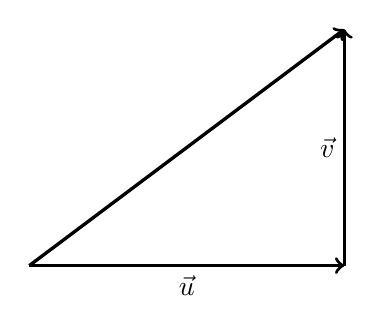
\begin{tikzpicture}
        \draw[->, very thick] (4,0) -- (4,3);
        \draw[->, very thick] (0,0) -- (4,0);
        \draw[->, very thick] (0,0) -- (4,3);
        \draw (2,0) node[anchor = north] {$\vec u$};
        \draw (4,1.5) node[anchor = east] {$\vec v$};
    \end{tikzpicture}
\end{center}
\[ ||\vec u + \vec v||^2 = ||\vec u||^2 + ||\vec v||^2 \iff \la \vec u + \vec v, \vec u + \vec v\ra = \la \vec u, \vec u \ra + \la \vec v, \vec v \ra \]
\end{theorem}
\begin{proof} We compute
    \[ \la \vec u + \vec v, \vec u + \vec v\ra = \la \vec u,\vec u \ra + \la \vec u , \vec v \ra + \la \vec v, \vec u \ra + \la \vec v,\vec v \ra = \la \vec u,\vec u \ra + 0 + 0 + \la \vec v,\vec v \ra = ||\vec u|| + ||\vec v|| \]
\end{proof}
\subsubsection*{Obeservation}
Given $\vec u,\vec v \in V$ such that $\vec v \neq 0$, we want to modify $\vec u$ such that $\vec u + c\vec v$ is orthogonal to $\vec v$. We know that $\la \vec v + c\vec v, \vec v \ra = 0$, solve for $c$ gives $c = \displaystyle\frac{-\la \vec u, \vec v\ra}{\la \vec v, \vec v \ra}$.
\begin{center}
    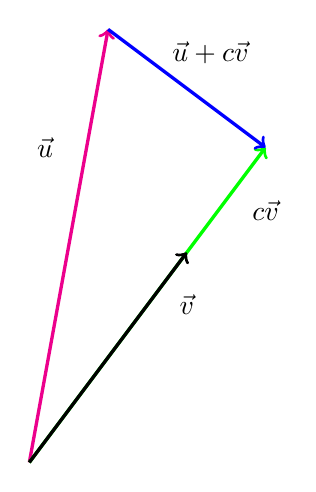
\begin{tikzpicture}
        \draw[->, very thick, color = magenta] (0,0) -- (1, 5.5);
        \draw[->, very thick, color = green] (0,0) -- (3, 4);
        \draw[->, very thick] (0,0) -- (2,2.66666666);
        \draw[->, very thick, color = blue] (1, 5.5) -- (3,4);
        \draw (2,2) node {$\vec v$};
        \draw (0.2,4) node {$\vec u$};
        \draw (3,3.2) node {$c\vec v$};
        \draw (2.3, 5.2) node {$\vec u + c\vec v$};
    \end{tikzpicture} 

    An orthogonal decompostion
\end{center}
\begin{theorem}[Cauchy-Schwarz Inequality]
    For any $u,v \in V$ where $V$ is a inner product space, the following holds
    \[ |\la \vec u,\vec v \ra| \leq ||\vec u|| \cdot ||\vec v||\]
\end{theorem}
\begin{proof}
    Given $\vec u,\vec v \in V$, we can assume without the loss of generality that $\vec v \neq 0$. So we can consider vectors $\vec u + c\vec v$ and $\vec v$ that are orthogonal for the choice that 
    \[ c: = \frac{ - \la \vec u,\vec v \ra}{\la \vec v,\vec v\ra}\]
    By Pathgrathrean theorem, $||\vec u + c\vec v||^2 + ||c\vec v||^2 = ||\vec u||^2$. But $||c\vec v||^2 = |c|^2||\vec v||^2$ and recall \[ c= \frac{- \la \vec u,\vec v\ra}{\la \vec v,\vec v\ra}, \text{ so } c^2= \frac{|\la \vec u, \vec v\ra|^2}{\la \vec v,\vec v\ra^2} = \frac{|\la \vec u, \vec v \ra|^2}{||\vec v||^4}, \text{ therefore } ||c\vec v||^2 = \frac{|\la \vec u, \vec v \ra|^2}{||\vec v||^4} ||\vec v||^2 = \frac{|\la \vec u, \vec v \ra|^2}{||\vec v||^2}\]
    So by dropping $||\vec u + c\vec v||^2 > 0$, we obtain $||c\vec v||^2 \leq ||\vec u||$, i.e, 
    \[ \frac{|\la \vec u, \vec v \ra|^2}{||\vec v||^2} \leq ||\vec u||^2 \implies |\la \vec  u,\vec v\ra|^2 \leq ||\vec u|^2 \cdot ||\vec v||^2 \implies |\la \vec u,\vec v \ra|^2 \leq ||\vec u|| \cdot ||\vec v||\]
\end{proof}
\begin{theorem}[Triangle Inequality]
\[ ||\mathbf u + \mathbf v|| \leq ||\mathbf u|| + ||\mathbf v||\]
\end{theorem}
\begin{proof}
 We have 
 \begin{align*}
    ||\vec u + \vec v||^2 &= \langle \vec u + \vec v, \vec u + \vec v \rangle = \la \vec u + \vec u \ra + \cg{\vec v, \vec v} + \cg{\vec u, \vec v} + \cg{\vec v, \vec u} \\
    &= ||\vec u||^2 + ||\vec v||^2 + \cg{\vec u + \vec v} + \bar{\cg{\vec u + \vec v}} = ||\vec u||^2 + ||\vec v||^2 + 2\text{Re}\cg{\vec u, \vec v} \\
    &\leq ||\vec u||^2 + ||\vec v||^2 + 2|\cg{\vec u, \vec v}| \leq ||\vec u||^2 + ||\vec v||^2 + 2||\vec u||\ ||\vec v|| \\
    &= \left(||\vec u|| + ||\vec v||\right)^2
 \end{align*}
\end{proof}
\begin{theorem}[Alternative Version of Triangle Inequality]
    \[ \big| ||\vec u|| - ||\vec v|| \big| \leq ||\vec u - \vec v||\]
\end{theorem}
\begin{proof}
    Notice that 
    \[   ||\vec u|| - ||\vec v|| \leq ||\vec u - \vec v|| \iff ||\vec u|| \leq ||\vec u - \vec v||  + ||\vec v||\]
    Which is the triangle inequaliy. Swapping out $\vec u$ and $\vec v$ gives us \[   ||\vec v|| - ||\vec u|| \leq ||\vec v - \vec u|| \iff ||\vec u|| \leq ||\vec u - \vec v||  + ||\vec v||\]
    Combining these equations gives us
    \[ \big| ||\vec u|| - ||\vec v|| \big| \leq ||\vec u - \vec v||\]
\end{proof}
\begin{fact}[Fun inequalities]
\[ ||\vec u + \vec v||^2 + ||\vec u + \vec v||^2 = 2\left(||\vec u||^2 + ||\vec v||^2\right)\]
\end{fact}
\subsection{Orthogonality}
\begin{definition}
    A list $\li{\vec v}{k}$ is $V$ is called orthonormal if \[ \la \vec v_i \vec v_j \ra = \delta_{ij} = \left\{\begin{array}{cc}
        1 & \text{if } i = j \\
        0 & \text{if } i \neq j \\
    \end{array} \right.\]
\end{definition}
\begin{lemma}
    Any list of orthonormal vectors is necessarily linearly indepedent.
\end{lemma}
\begin{proof}
    Suppose $\lincomb{\alpha}{\vec v}{k} = \vec 0$. We can compute on the standard inner product
    \[ \la \lincomb{\alpha}{\vec v}{k} , \vec v_1 \ra = \alpha_1 \la \vec v_1, \vec v_1 \ra + \alpha_2 \la \vec v_2, \vec v_1 \ra + \cdots + \alpha_k \la \vec v_k, \vec v_1 \ra \implies \alpha_1 = 0\]
    \[ \la \lincomb{\alpha}{\vec v}{k} , \vec v_2 \ra = \alpha_1 \la \vec v_2, \vec v_2 \ra + \alpha_2 \la \vec v_2, \vec v_2 \ra + \cdots + \alpha_k \la \vec v_k, \vec v_2 \ra \implies \alpha_1 = 0\]
    \[ \vdots \]
    \[ \la \lincomb{\alpha}{\vec v}{k} , \vec v_k \ra = \alpha_1 \la \vec v_1, \vec v_k \ra + \alpha_2 \la \vec v_2, \vec v_k \ra + \cdots + \alpha_k \la \vec v_k, \vec v_k \ra \implies \alpha_k = 0\]
    Hence $\li{\vec v}k$ is linearly indepedent.
\end{proof}
\begin{question}
    What is nice about orthonormal basis?
\end{question}
\begin{answer}
    If $(\li{\vec v}n)$ is an orthonormal basis, then an arbitary vector can be written as 
    \[ \vec v = \la \vec v, \vec v_1 \ra \vec v_1 + \la \vec v, \vec v_2 \ra \vec v_2 + \cdots + \la \vec v, \vec v_n \ra \vec v_n\]
    Furthermore, we can conclude the following theorem:
\end{answer}
\begin{theorem}[Generalized Pythagorean Theorem]
\[ ||\vec v||^2 = \sum_{j = 1}^{n} \big| \la \vec v, \vec v_j \ra \big|^2\]
\end{theorem}
\begin{algorithm}[Gram-Schmidt Algorithm]
    \texttt{Input}: Any $\li{\vec v}m$ that is linearly independent. \\
    \texttt{Output}: $\li{\vec e}m$ such that $\vec e_j \in \spa (\li{\vec v}j)$ for all $j \leq n$.
    \begin{proof}[Process] $ $
        \begin{align*}\vec e_1 &= \frac{\vec v_1}{||\vec v_1||} \\
        \vec e_2 &= \frac{\vec v_2 - \la \vec v_2, \vec e_1 \ra \vec e_1}{||\vec v_2 - \la \vec v_2, \vec e_1 \ra \vec e_1||} \\
        \vec e_3 &= \frac{\vec v_3 - \la \vec v_3, \vec e_1 \ra \vec e_1 - \la \vec v_3, \vec e_2 \ra \vec e_2}{||\vec v_3 - \la \vec v_3, \vec e_1 \ra \vec e_1 - \la \vec v_3, \vec e_2 \ra \vec e_2||} \\
        \vdots \\
        \vec e_n &= \frac{\vec v_n - \la \vec v_{n}, \vec e_1 \ra \vec e_1 - \la \vec v_n, \vec e_2 \ra \vec e_n \cdots - \la \vec v_n - \vec e_{n-1} \ra \vec e_{n-1}}{||\vec v_n - \la \vec v_{n}, \vec e_1 \ra \vec e_1 - \la \vec v_n, \vec e_2 \ra \vec e_n \cdots - \la \vec v_n - \vec e_{n-1} \ra \vec e_{n-1}||}
        \end{align*}
    \end{proof}
\end{algorithm}
\begin{proposition}
    Every finite inner product vector space has a orthonormal basis. 
\end{proposition}
\begin{proof}
    Suppose $V$ is a finite dimensional vector space. Let $\li{\vec v}n$ be a basis for $V$. We then apply Gram-Schmidt Algorithm to the basis to obtain a orthonormal basis $\li{\vec e}n$. 
\end{proof}
\begin{remark}[Projection orthonal with the repect to inner product]
    Given a subsace $U$ of $V$ for finie dimensioanl vector space $V$, there is a projector $P_V$ that project all vectors in $V$ on $V$ orthogonally.
\end{remark}
\begin{remark}[Relations between inner product and linear functionals]
    Suppose $V$ is finite dimensional vector space. Given any $\vec u \in V$, then function $\la \cdot, \vec u\ra$ is a linear functional (i.e. an element of $V' = \c L(V,\b F)$)
\end{remark}
\begin{theorem}[Riesz Representation Theorem]
    For any $\varphi \in V'$ there exists a \textit{unique} $\vec u \in V$ such that $\la \vec v, \vec u \ra = \varphi (\vec v) = \varphi(\vec v)$ for al $\vec v \in V$.
\end{theorem}
\newpage
\begin{proof} \textbf{Existence} \\
    Take an orthonormal basis $\li{\vec v}n$. of $V$. Any $\vec v$ can be written as a linear combination the basis (To preserve linearity we want to put $\vec v$ into the first slot)
    \begin{align*} \vec v &= \la \vec v , \vec e_1 \vec \ra \vec e_1 + \la \vec v, \vec e_2 \ra + \cdots + \la \vec v, \vec e_n \ra \\
    \varphi(v) &= \la \vec v , \vec e_1 \vec \ra \varphi(\vec e_1) + \la \vec v, \vec e_2 \ra \varphi(\vec e_2)+ \cdots + \la \vec v, \vec e_n \ra \varphi(\vec e_n) \\
    &= \la \vec v + \bar{\varphi(\vec e_1)}e_1 + \bar{\varphi(\vec e_2)}e_2 + \cdots + \bar{\varphi(\vec e_n)}\vec e_n \ra \\ 
    &= \vec u 
    \end{align*}
    \textbf{Uniqueness} \\
    Suppose there are $\vec u_1, \vec u_2$ such that $\la \vec v, \vec u_1 \ra = \la \vec v, \vec u_2 \ra$ for all $\vec v \in V$. Take $\vec v = \vec u_1 - \vec u_2$. We can see that 
    \[ \la \vec v_1, \vec u_1 \ra + \la \vec v, \vec v_2 \ra \iff \la \vec v, \vec u_1 - \vec u_2 \ra\]
    Plug in $v$ and we get 
    \[ \la \vec u_1 - \vec u_2, \vec u_1 - \vec u_2 \ra = ||\vec u_1 - \vec u_2||^2 = 0\]
    This means that $\vec u_1 - \vec u_2 = 0$, or $\vec u_1 = \vec u_2$, hence such $\vec u$ is unique.
\end{proof}
\begin{example}
    Let $V := \c P(\b C)$ and let $\displaystyle \varphi(p) := \int_{-1}^1 p(t) \sin t \cdot dt$. Find a reprsentation in $V$ with with respect to
    \[ \la f,g \ra = \int_{-1}^1 f(t) \bar{g(t)} dt\] 
    Suppose $p(t) = a_0 + a_1t + a_2t^2$.
\end{example}
\subsection{Orthogonality and Orthogonal Projections}
\begin{definition}
    Given an inner produce space $V$ and its subset $U$ of $V$ we can define 
    \[ U^\perp := \b \vec v \in V : \lb \vec u , \vec v \ra = 0 \ \forall \vec u \in U \rb \]
\end{definition}
\begin{theorem}
Basic facts about orthogonal complement
\begin{enumerate}[label = (\alph*)]
    \item If $U$ is a susbet of $V$, then $U^\perp$ is a subspace of $V$.
    \item $\lb \vec 0 \rb^\perp = V$
    \item $V^\perp = \lb \vec 0 \rb$
    \item $U \cap U^\perp \subseteq \lb \vec 0 \rb$ 
    \item If $U \subseteq W$ then $U^\perp \supseteq W^\perp$
\end{enumerate}
\end{theorem}
\begin{proof} $ $
\begin{enumerate}[label = (\alph*)] 
    \item Clearly $\vec 0 \in U^\perp$ as $\la \vec v, \vec 0 \ra = 0 \ \forall \vec v \in V$. Take $\vec v_1, \vec v_2 \in U^\perp$ and $\lambda \in \b F$, then $\la \vec v_1 + \lambda \vec v_2, \vec u \ra = \la \vec v_1, \vec u \ra + \lambda \la \vec v_2, \vec u \ra = 0 \ \forall \vec u \in U$.
    \item Trivial by part (c).
    \item Trivial by part (b).
    \item Suppose $\vec v \in U \cap U^\perp$, then $\la \vec v, \vec v \ra = 0 \implies \vec v = \vec 0$.
    \item Suppose $\vec v \in W^\perp$, then $\la \vec v, \vec w \ra = 0 \ \forall \vec w \in W$. Since $U \subseteq W$, $\la \vec v, \vec u \ra = 0 \ \forall \vec u \in U$, hence $U^\perp \supseteq W^\perp$.
\end{enumerate}
\end{proof}
\begin{theorem}
    If $V$ is a finite dimensional inner product space and $U$ is a subspace of $V$, then \[U \oplus U^\perp = V\]
\end{theorem}
\begin{proof}
    We already know that the sum is direct by $U \cap U^\perp = \lb 0 \rb$.  By Gram Schmidt we can construct an orthonormal basis of $U$ and extend it to a normal normal basis of $V$ we have $\li{\vec u}k, \li{\vec v}n$. We claim that $\li{\vec v}n$ is a basis of $U^\perp$ as $\la \vec u_i, \vec v_j \ra = 0$ for all $i$ in $1,2, \ldots, k$ and $j$ in $1,2, \ldots, n$. Hence $\li{\vec v}n \in U^\perp$. On the other hand, 
    \[ U^\perp \in \lincomb{\alpha}{\vec u}k + \lincomb{\beta}{\vec v}{n} \]
    must satisify $\alpha_j = \la \vec v_i, \vec u_j \ra = \vec 0$ for all $i$ in $1,2, \ldots, k$. Therefore we have $U^\perp = \spa (\li{\vec v}n)$. Hence $U \oplus U^\perp = V$.
\end{proof} \vfill
%!TEX root = ./main.tex
\section{Operators on Inner Product Spaces}
\subsection{Self-Adjoint and Normal Operators}
\begin{definition}
	Suppose $T \in L(V,W)$, we define $T*$ by this formula 
	\[ \la T\vec v, \vec w \ra_W = \la \vec v, T^* \vec w \ra_V\]
\end{definition}
We can think og $\vec w$ as fixed, we note that $\la T \ast, \vec w \ra$ is a linear functiona;. hence it has a representer by Riesz, so we are entitled to call it $T^*\vec w$ such that 
\[ \la T\vec v, \vec w \ra = \la \vec v, T^* \vec w \ra \]
Hence we have $T^* \in \c L(W,V)$. We want to verify this property. Consider $T*(\vec w_1 + \lambda \vec w_2)$. We compute 
\begin{align*}
	\la \vec v, T*(\vec w_1 + \lambda \vec w_2) \ra &= \la T\vec v, \vec w_1 + \lambda \vec w_2\ra \\
	&= \la T\vec v, \vec w_1 \ra + \bar \lambda \la T\vec v + \vec w_2 \ra \\
	&= \la \vec v, T^*\vec w_1 \ra +  \bar \lambda \la \vec v, T^* \vec w_2 \ra \\
	&= \la \vec v, T^*\vec w_1 \ra +   \la \vec v, \lambda T^* \vec w_2 \ra \\
	&= \la \vec v, T^*\vec w_1 +  \lambda T^*w_2 \ \ra \forall \vec v \in V, \vec w_1, \vec w_2 \in W, \lambda \in \b F 
\end{align*}
So $T^*(\vec w_1 + \lambda \vec w_2) = T^* \vec w_1 + \lambda T^* \vec w_2$.

\begin{theorem}[Properties of the adjoint]
Let $T \in \c L(V,W)$, we have
	\begin{enumerate}
		\item $(S + T)^* = S^* + T^*$
		\item $(\lambda T)^* = \bar \lambda T^*$
		\item $(S \cdot T)^* = T^*S^*$
		\item $(\lambda T)^* = \bar \lambda T^*$
		\item $\b I^* = \b I$
	\end{enumerate}
\end{theorem}
\begin{proof} TODO: Refer to book page 206
\end{proof}
\begin{theorem}[Null space and range of adjoint]
Let $T \in \c L(V,W)$, then
	\begin{enumerate}
		\item $\nul T^* = (\range T)^\perp$
		\item $\range T^* = (\nul T)^\perp$
		\item $\nul T = (\range T*)^\perp$
		\item $\range T = (\nul T^*)^\perp$
	\end{enumerate}
\end{theorem}
\begin{proof}
Let $\vec w \in W$. Then 
\begin{align*}
	\vec w \in \nul T^* &\iff T^* \vec w = 0 \\
	&\iff \la \vec v, T^* \vec w \ra = 0 \ \forall \vec v \in V \\
	&\iff \la T\vec v, \vec w \ra \ \forall \vec v \in V \\
	&\iff \vec w \in (\range T)^\perp
\end{align*}
(b),(c),(d) follows by a similar logic and is left as an exercise.
\end{proof}

\begin{definition}
Let $T \in \c L(V)$. $T$ is called self-adjoint if $T^* = T$.
\end{definition}
\begin{definition}
	$T$ is called normal if $TT^* = T^*T$.
\end{definition}
%\begin{example}
%	Let $V$ be $\b R^3$ with the standard inner product, let $T \in \c L(V)$ such that $T: (x_1,x_2,x_3) \mapsto (x_1,2x_2,3x_3)$.
%\end{example}
\begin{example}
	Suppose $T \in \c L(V)$, we can define $T: \vec v \mapsto \la \vec , \vec x \ra \vec y$ for some fixed $\vec x, \vec y$ in $V$. Compute $T^*$. \\
	We compute 
	\begin{align*}
		\langle \vec v, T^* \vec w \rangle &= \langle T \vec v, \vec w \rangle  \\
		&= \langle \langle \vec v, \vec x \rangle \vec y, \vec w \rangle  \\
		&= \langle \vec v, \vec x \rangle \langle \vec y, \vec w \rangle \\
		 &= \langle \vec v, \overline{\langle \vec y, \vec w \rangle} \vec x \rangle \\
		 &= \langle \vec v, \langle \vec w, \vec y \rangle \vec x \rangle
	\end{align*}
	hence we can concldue $T^* \vec w = \la \vec w, \vec y \ra \vec x$ for all $\vec w \in W$.
\end{example}
\newpage
\subsubsection{Matrix representation}
Suppose $T \in \c L(V,W)$, where $V,W$ are finite-dimensional vector spaces. Let $\li{\vec e}n$ be an orthonormal basis for $V$ and $\li{\vec f}m$ be a orthonormal basis for $W$. We can see that $\c M(T)$ is obtained through
\[ T \vec e_j = \la T\vec e_j, \vec f_1 \ra \vec f_1 + \la T\vec e_j, \vec f_2 \ra \vec f_2 + \cdots + \la T\vec e_j, \vec f_m \ra \vec f_m\]
\[ T^* \vec f_k = \la T^* \vec f_k, \vec e_1 \ra \vec e_1 + \la T^* \vec f_k, \vec e_2 \ra \vec e_2 + \cdots + \la T^* \vec f_k, \vec e_n \ra \vec e_n\]
Then 
\[ \c M(T^*)(l,k) = \la T^* \vec f_k, \vec e_l \ra \implies \c M(T^*)(j,i) = \la T^* \vec f_i, \vec e_j \ra \]
Therefore we have $\c M(T^*) = \bar{\c M(T)}^T$
\begin{remark}
	The above statement only holds if the basis for $V$ and $W$ are orthonormal.
\end{remark}
\begin{remark}
	If an operator $T$ is self-adjoint, then $T$ is normal, but not the converse.
\end{remark}

\begin{proposition}
	The eigenvalue of any self-adjoint operator is real.
\end{proposition}
\begin{proof}
Suppose self-adjoint $T \in \c L(V)$. and $\lambda$ is an eigenvalue of $T$ and let $\vec v$ be the eignevector corespond to $\lambda$. We compute 
\[
	\lambda \la \vec v, \vec v \ra = \la \lambda \vec v, \vec v \ra 
	= \la T\vec v, \vec v \ra 
	= \la \vec v, T\vec v \ra 
	= \la \vec v, \lambda \vec v \ra 
	= \bar \lambda \la \vec v, \vec v \ra
\] We can see that $\lambda = \bar \lambda \implies \lambda \in \b R$.
\end{proof}
\begin{question}
	Suppose $\la T\vec v,\vec v \ra = 0 \forall \vec v \in V$. Does the statement implies $T$ is the zero map?
\end{question}
\begin{answer}[Surprisingly]
	Yes over $\b C$ and no over $\b R$.
\end{answer}
\begin{proof}
	Supoose $\b F = \b C$, the following holds.
	\[ \la T(\vec v + \vec w), \vec v + \vec w \ra = \la T\vec v, \vec v \ra + \la T\vec v, \vec w \ra + \la T\vec w,\vec v \ra + \la T\vec w, \vec w \ra \]
	\[ \la T(\vec v - \vec w), \vec v + \vec w \ra = \la T\vec v, \vec v \ra - \la T\vec v, \vec w \ra - \la T\vec w,\vec v \ra + \la T\vec w, \vec w \ra \]
	Subtratc the first equation by the second we have 
	\[ \la T(\vec v + \vec w), (\vec v + \vec w) \ra - \la T(\vec v - \vec w), (\vec v + \vec w) \ra =\boxed{ 2\la T\vec v, \vec w\ra + 2\la T\vec w, \vec v \ra} \]
	We also compute 
	\[ \la T(\vec v + i\vec w) , (\vec v + i\vec w)\ra - \la T(\vec v - i\vec w) , (\vec v - i\vec w)\ra = \boxed{2i\left(\la T\vec w, \vec v\ra - \la T\vec v, \vec w \ra\right)}\]
	Take the two boxed equation and divide the second one by $i$ then subtract from first gives us 
	\[ 4\la T \vec v, \vec w \ra = 0\]
	Suppose $\b F = \b R$. Consider $\b R^2$. Take $T\vec v$ and rotate $\pi / 2$ gives us $T(x_1, x_2) := (-x_2 , x_1)$. We can see that $\la T\vec v, \vec v \ra = 0 \forall \vec v$ but $T \neq 0$. However, if $T$ is self-adjoint then $T$ is $0$.
\end{proof}
\begin{remark}
	Suppose $\b F = \b R$ and $T = T^*$. We have 
	\[ 4\la T\vec v, w \ra = \la T(\vec v + \vec w), (\vec v + \vec w) \ra - \la T(\vec v - \vec w), (\vec v - \vec w )\ra\]
	Hence $T = 0$. 
\end{remark}

\begin{corollary}
	$\la T \vec v, \vec v \ra \in \b R$ in a complex space is equivalent to $T$ being self adjoint.
\end{corollary}
\begin{proof}
	\[ \la T \vec v, \vec v \ra \in \b R \iff \la T\vec v, \vec v\ra = \la T^*\vec v, \vec v \ra \implies \la (T - T^*)\vec v, \vec v\ra = 0 \implies T - T^* = 0\]
	We can see that $T = T^*$. Hence $T$ is self-adjoint.
\end{proof}

\begin{theorem}
	$T$ is normal if anf only if $||T\vec v|| = ||T^* \vec v|| \ \forall \vec v \in V$.
\end{theorem}
\begin{proof}
	\[ ||T\vec v|| = ||T^* \vec v|| \implies \la T\vec v, T\vec v\ra = \la T^* \vec v, T^* \vec v \ra \implies \la T^* T \vec v, \vec v \ra = \la TT^* \vec v, \vec v \ra\]
	Hence $T$ is normal sicne $TT^* = T^*T$.
\end{proof}
\begin{theorem}
	Say $\lambda, \vec v$ is an eigenpair of a normal oeprator $T$, then 
	\[ ||(T - \lambda \b I) \vec v ||=||(T^* - \bar \lambda \b I)\vec v||\]
\end{theorem}

 \vfill
%!TEX root = ./main.tex
\section{Operators on Complex Vector Spaces}
\setcounter{subsection}{2}
\subsection{Characteristic and Minimal Polynomial}
\begin{definition}
	The number of times an eignevalue $\lambda$ appears in the matrix is called the algebragic multiplicity of $\lambda$.
\end{definition}
\begin{example}
	Suppose $V$ is a complex vector space and let $T \in \c L(V)$. Supppose $T$ has the following matrix presentation
\[ \bml 
	2 & 1 & 0 \\
	0 & 2 & 1 \\
	0 & 0 & 2 \\
	&&& 3 & 1 \\
	&&& 0 & 3 \\
	&&&&& 2	\bmr\]
	We can see that $\lambda = 2$ has a multiplicity of $4$ and $\lambda = 3$ has a algebraic multiplicaity of $2$.
\end{example}
\begin{definition}
	Suppose $V$ is a complex vector space and $T \in \c L(V)$. Suppose $T$ has eigenvalues $\li \lambda n$ with algebraic multiplicity of $\li dn$. Then the polynomial
	\[ p_{\text{char}}(z) = \prod_{j} (z - \lambda_j)^{d_j} \] is the characteristic polynomial of $T$.
\end{definition}
\begin{theorem}[The Cayley-Hamilton Theorem]
	Suppose V is a complex vector space and $T \in \c L(V)$. Then $p(T) = 0$, where $p$ is the characteristic polynomial. 
\end{theorem}
\begin{proof}
	Trivial by Jordan Normal Form in section 8.d.
\end{proof}	
\begin{definition}
	A minimal polynomial for $T \in \c L(V)$ os a monoic polynomial of the smallest degree that annihilates $T$. i.e. $q(T) = 0$ and $q$ is of smallest degree with this property of leading coefficient $1$.
\end{definition}
\begin{example}
	Consider $T$ in example 8.2. Take the largest block of eahc eigenvalue and raise each term to the size of the block will yield the minimal polynomial
	\[ p_{text{min}} (z) = (z - 2)^3(z - 3)^2\]
\end{example}
\begin{corollary}
	Suppose $h(T) = 0$ for some polynomial $h \not\equiv 0$. Then $h(z) = p_{\text{min}} (z)q(x)$ for some $q$.
\end{corollary}
\begin{proof}
	By the remainder theorem we have 
	\[ h(z) = p_{\text{min}}(z)q(z) + r(z)\]
	where $\deg r < \deg p_{\text{min}}$. By the minimality of $p_{\text{min}}$, $r \equiv 0$.
\end{proof}
\subsection{Jordan Form}
\subsubsection*{Goal} To find te the sparest matrix representation for an arbitary linear operator on a finite dimensional vector space over $\b C$.
\subsubsection{Observation}
``Rough'' decomposition 1
\[ \left[\begin{array}{ccc|ccc} 
\ast & \cdots & \ast & 0 & \cdots & 0 \\ 
\vdots & \ddots & \vdots & \vdots & \ddots & \vdots \\ 
\ast & \cdots & \ast & 0 & \cdots & 0 \\
\hline
0 & \cdots & 0  & \ast & \cdots & \ast  \\ 
\vdots & \ddots & \vdots & \vdots & \ddots & \vdots\\ 
0 & \cdots & 0 & \ast & \cdots & \ast \\

          \end{array}\right]  = \c M(T)\]
          Notice that $T$ has two invariant subspaces that are direct sums of each other.
\begin{definition}
	An operator is called nilpotent if some power of it equals to $0$.
\end{definition}
\begin{proposition}
	For any $T \in \c L(V)$, there exists two subsapces, $V_s$ and $V_r$ such that $V = V_s \oplus V_r$ and $V_s,V_r$ are both $T$-invariant, and $T\vert_{V_s}$ is nilpotent and $T\vert_{V_r}$ is invertible. 
\end{proposition}

\begin{proof}
Consider 
\[ \lb v \rb \subseteq \nul T \subseteq \nul T^2 \subseteq \cdots\]
Because $\dim V \leq \infty$, we must be able to find $q \in \b N$ such that $T^q$ and $T^{q+h}$ for any $h \in \b N$ have the same null space. In other words 
\[ \exists q\in \b N : \nul T^q = \nul T^{q + h} \qquad \forall k \in \b N\]
Take $V_s : = \nul T^q$ and $V_r = \range T^q$. Obsrve that $V_s$ and $V_r$ ae $T$-invariant. 

\noindent Next we want to check that $V_s \cap V_r = \lb \vec 0 \rb$. \\ 
Suppose $\vec v \in V_s \cap V_r$. Then $T^q \vec v = \vec 0$, and $T^q \vec w = \vec v$ for some $\vec w \in V$. So $T^{2q}\vec w = \vec 0$. Hnec eby the choice of $q$ we have $\vec w \in \nul T^q$, so \[T^q \vec w = \vec 0 = \vec v\]
So $\vec v = 0$, and $V_s \cap V_r = \lb \vec 0 \rb$. By Rank-Nullity, $V = V_s \oplus V_r$. \\
$T\vert_{V_s}$ is nilpotent sicne $\left(T\vert_{V_s}\right)^2$ is zero. \\
$T\vert_{V_r}$ is invertible since for any $\vec w \in V_r$ such that $T \vec w = \vec 0$ will also satify $T^q \vec w = \vec 0$, hence $\vec w = \vec 0$, and $T\vert_{V_r}$ being injective implies invertiablity.
\end{proof}
\subsubsection*{Zoom in to the nilpotent part}
	Say, the whole space $V$ satifies the condition $T^q = 0$ and without the loss of generality we can take $q$ minimal with this property. This means there exists $\vec v_0 \in V$ such that $T^{q - 1} \vec v_0 \neq \vec 0$. Take 
	\[ \vec v_0 = \spa \lb \vec v_0 , T\vec v_0, \ldots, T^{q-1} \vec v_0 \rb\]
	Since there exists a vector such that $T^{q - 1} \vec v_0 \neq \vec 0$ we can also there exists $\vec w_0 \in V$ such that $\la T^{q-1}\vec v_0, \vec w_0\ra \neq 0$. Take the following matrix
	\[ \left( \la T^{j-1}\vec v_0 , T^{*^{q-i}} \vec w_0 \ra\right)_{i,j = 1}^q = \left( \la T^{q + j - i - 1} \vec v_0, \vec w_0 \ra\right)_{i,j = 1}^q\]
	Notice that this is a lower triangular matrix with nonzero diagonal matrix.
\begin{corollary}
	The list $\vec v_0 , T\vec v_0, \ldots, T^{q-1} \vec v_0$ is linearly indepedent and so is the list $\vec w_0 , T^*\vec w_0, \ldots, T^{*^{q-1}} \vec w_0 $
\end{corollary}
\begin{proof}
	Take $V_1 := \left( \spa \left( \vec w_0 , T^*\vec w_0, \ldots, T^{*^{q-1}} \vec w_0 \right) \right)^{\perp}$. Notice that if $W$ is $T*$-invariant, $W^\perp$ is $T$-invariant. Indeed, for any $\vec v \in W^\perp$ and any $\vec w \in W$, we have \[\la T \vec v, \vec w \ra =\la  \vec v, T^* \vec w \ra = 0\]
	Hence we have $V = V_0 \oplus V_1$, where $V_0, V_1$ are both $T$-invariant. To see that the sum is direct 
	Suppose \[\alpha_0 \vec v_0 + \alpha_1 T\vec v_0 + \cdots + \alpha^{q-1}T^{q-1}\vec v\]
	is orthogonal to $\vec w_0 , T^*\vec w_0, \ldots, T^{*^{q-1}} \vec w_0 $. Thn the matrix 
	\[ \left( \la T^{j-1} \vec v_0, T^{*^{q-1}} \vec w_0 \ra\right)\] 
	being invertible gurantees that
	\[ \alpha_0 = \alpha_1 = \cdots = \alpha_{q-1} = 0\]
\end{proof}
\subsubsection*{fine decomposition}
We look at $\c M\left( T\vert_{V_1}\right)$ with respect to the basis $\vec v_0 , T\vec v_0, \ldots, T\vec v_0$. Hence we have 
\[ \bml 
	0 & 0 & 0 & \cdots & 0 & 0\\ 
	1 & 0 & 0 & \cdots & 0 & 0\\
	0 & 1 & 0 & \cdots & 0 & 0\\
	\vdots & \vdots & \vdots & \ddots & \vdots & \vdots\\

	0 & 0 & 0 & \cdots & 1 & 0\bmr\]
\subsubsection*{Warp-up}
Repeat the process many gives 
\[V = V_1 \oplus V_2 \oplus \cdots \oplus V_n \]
This guarantees a bock-diagonal form where each block looks like 
\[ \bml 
\lambda_j & 1 \\	
& \lambda_j & 1 \\
&& \lambda_j & 1 \\
&&& \lambda_j & 1 \\
&&&& \ddots & \ddots \\
&&&&& \lambda_j & 1 \\
&&&&&& \lambda_j
\bmr\]


\begin{example}
	Consider
	\[ \c M(T) =  \bml 
		3 & 1 & 0 & 0 & 0 & 0 & 0 & 0 & 0 & 0 & 0 & 0\\
		0 & 3 & 1 & 0 & 0 & 0 & 0 & 0 & 0 & 0 & 0 & 0\\
		0 & 0 & 3 & 0 & 0 & 0 & 0 & 0 & 0 & 0 & 0 & 0\\
		0 & 0 & 0 & 3 & 1 & 0 & 0 & 0 & 0 & 0 & 0 & 0\\
		0 & 0 & 0 & 0 & 3 & 0 & 0 & 0 & 0 & 0 & 0 & 0\\
		0 & 0 & 0 & 0 & 0 & 3 & 0 & 0 & 0 & 0 & 0 & 0  \\
		0 & 0 & 0 & 0 & 0 & 0 & -2 & 1 & 0 & 0 & 0 & 0 \\
		0 & 0 & 0 & 0 & 0 & 0 & 0 & -2 & 0 & 0 & 0 & 0 & \\
		0 & 0 & 0 & 0 & 0 & 0 & 0 & 0 & 1 & 1 & 0 & 0\\
		0 & 0 & 0 & 0 & 0 & 0 & 0 & 0 & 0 & 1 & 0 & 0\\
		0 & 0 & 0 & 0 & 0 & 0 & 0 & 0 & 0 & 0 & 0 & 1 \\
		0 & 0 & 0 & 0 & 0 & 0 & 0 & 0 & 0 & 0 & 0 & 0 \bmr\]
Where the empty entries are zero. We can see that the $T$ has eigenvalue $3,-2,1,0$. \\
We can see that \begin{align*} \dim \nul (T - 3 \b I)^j &= 3,5,6,6,6, \ldots \\
\dim \nul (T + 2\b I)^j &= 1,2, \ldots \\
\dim \nul (T - 1 \b I)^j &= 1,2,2,\ldots \\
\dim \nul (T - 0 \b I)^j &= 1,2,2,2, \ldots \\
j = 1,2,3, \ldots & \qquad \forall\ j \in \b N
\end{align*}
\end{example}
\begin{example}
	Suppose $V:= \c P_4(\b C)$. Let $D$ be the differetiation operator. Construct the Jordan Normal Form of $D$ and the Jordan Basis of $V$. \\
	We can compute for $\c M(T)$ with the standard basis
	\[ \bml 
		0 & 1 & 0 & 0 & 0 \\
		0 & 0 & 2 & 0 & 0 \\
		0 & 0 & 0 & 3 & 0 \\
		0 & 0 & 0 & 0 & 4 \\
		0 & 0 & 0 & 0 & 0 		
	\bmr\]
	with some algebraic manipulation we then can see that $D$ has jodran normal form of
	\[ \bml 
		0 & 1 & 0 & 0 & 0 \\
		0 & 0 & 1 & 0 & 0 \\
		0 & 0 & 0 & 1 & 0 \\
		0 & 0 & 0 & 0 & 1 \\
		0 & 0 & 0 & 0 & 0 		
	\bmr\]
	with basis $\displaystyle 1, x, \frac 12 x^2, \frac 13 x^3, \frac 14 x^4$.
\end{example}
\begin{example}
	Suppose $V = \spa \left( e^{ikt} : |k| \leq 3 \right)$. Let $D$ be the differetiation operator. Construct the Jordan Normal Form of $D$ and the Jordan Basis of $V$. \\
	We can see that $V = \spa (e^{-i3t},e^{-i2t},e^{-it},e^{0},e^{it},e^{i2t},e^{i3t})$. We can compute for the matrxi representation with repsect to the standard basis
	\[ \c M(T) = \bml 
	-3 \\
	& -2 \\
	&& -1 \\
	&&& 0 \\
	&&&& 1 \\
	&&&&& 2 \\
	&&&&&& 3 
	\bmr\]
	Notice that if we use basis $\displaystyle V = \spa \left(\frac{1}{-3i} e^{-i3t}, \frac{1}{-2i}e^{-i2t},\frac{1}{-i}e^{-it}, e^{0}, \frac{1}{i}e^{it}, \frac{1}{2i}e^{i2t}, \frac{1}{3i}e^{i3t}\right)$ we can obtain the Jordan Normal Form
	\[ \bml 1 \\
	& 1 \\
	&& 1 \\
	&&& 0 \\
	&&&& 1 \\
	&&&&& 1 \\
	&&&&&& 1 \bmr\]
\end{example}
\newpage
\subsubsection*{Reverse Engineering of the Jordan Normal Form}
\[ \begin{array}{|c|c|c|c|c|c|}
\hline 
& \dim (T - \lambda \b I) & \dim (T - \lambda \b I)^2 & \dim (T - \lambda \b I)^3 & \dim (T - \lambda \b I)^4 & \dim (T - \lambda \b I)^j, j \geq 5 \\
\hline
\hline 
\lambda = i & 3 & 6 & 7 & 7 & 7 \\
\lambda = -i & 2 & 4 & 6 & 8 & 8 \\
\lambda = 1 & 1 & 2 & 3 & \not5 \ \ 4 & 5 \\
\hline
\end{array}\]
What is the Jordan Normal form og $T$ based on this info? Assume all eigenvalues of $T$ are given above.
\begin{proof}[Solution] Notice that the difference in the sequence denotes the number of $1$'s that get send to $0$, hence we have the following matrix

\[ \bml 
	i & 1\\
	& i & 1\\
	&& i \\
	&&& i & 1\\
	&&&& i \\
	&&&&& i & 1\\
	&&&&&& i \\
	&&&&&&& -i & 1 \\
	&&&&&&&& -i & 1 \\
	&&&&&&&&& -i & 1 \\
	&&&&&&&&&& -i  \\
	&&&&&&&&&&& -i & 1 \\
	&&&&&&&&&&&& -i & 1 \\
	&&&&&&&&&&&&& -i & 1\\
	&&&&&&&&&&&&&& -i \\
	&&&&&&&&&&&&&&& 1 & 1 \\
	&&&&&&&&&&&&&&&& 1 & 1 \\
	&&&&&&&&&&&&&&&&& 1 & 1 \\
	&&&&&&&&&&&&&&&&&& 1 & 1 \\
	&&&&&&&&&&&&&&&&&&& 1 \bmr\]
\end{proof}
 \vfill
\begin{center} 
    Last updated: \today
\end{center}


 
%\include{chap9} \vfill
%\include{chap10} \vfill
%\thispagestyle{empty}
\setlist[enumerate,2]{leftmargin = 2cm}
\section*{Additional Materials}
\subsection*{Midterm 1}
\begin{enumerate}
    \item $\li vm$ be linear independent in $V$, find $\dim \spa (v_1 - v_2, v_2 - v_3, \ldots, v_{n-1} - v_n, v_n - v_1)$. 
    \begin{proof}
        Let $U = \spa ( v_1 - v_2, v_2 - v_3, \ldots, v_{n-1} - v_n, v_n - v_1 )$
        Notice that $v_1 - v_2, v_2 - v_3, \ldots, v_{n-1} - v_n, v_n - v_1$ is linearly independent, we guess that $\lb v_1 - v_2, v_2 - v_3, \ldots, v_{n-1} - v_n, v_n - v_1 \rb$ is a basis for $U$. 
        \begin{enumerate} [label = \textit{Step \arabic*.}]
                \item We want to show that $ v_1 - v_2, v_2 - v_3, \ldots, v_{n-1} - v_n$ is linearly independent. Suppose the equation  $a_1(v_1 - v_2) + a_2(v_2 - v_3) + \cdots + a_{n-1} (v_{n-1} - v_n) = 0\\ \implies a_1 v_1  + (a_2 - a_1) v_2 + \cdots + (a_{n-1} - a_n)v_{n-1} - a_{n-1} v_n = 0$. Since $\li vn$ is linearly independent, we know that $a_1 = a_2 - a_1 = \cdots = a_{n - 2} - a_{n_2} = a_{n-1} = 0 \implies \\ a_1 = a_2 = \cdots = a_{n-1} = 0$. Hence linear independence.
                \item We want to show that $U = \spa \lb  v_1 - v_2, v_2 - v_3, \ldots, v_{n-1} - v_n \rb$ 
                \begin{align*}
                    U &= c_1(v_1 - v_2) + c_2(v_2 - v_3) + \cdots + c_n(v_n - v_1) \\
                    &= c_1(v_1 - v_2) + \cdots + c_n(v_{n-1} - v_n) + c_n[-(v_1 - v_2) - \cdots - (v_{n-1} - v_n)] \\
                    &= (c_1 - c_n)(v_1 - v_2) + \cdots + (c_{n - 1} - c_n)(v_{n-1}v_n) \\
                    &= \spa \lb  v_1 - v_2, v_2 - v_3, \ldots, v_{n-1} - v_n \rb
                \end{align*}
        \end{enumerate}
    \end{proof}
    \begin{proof}[Alternative Proof.]
        Consider $T \in \b F^n \to \b F^n$ be defined as \[T(v_1) = v_1 - v_2, T(v_2) = v_2 - v_3, \ldots, T(v_n) = v_n - v_1\] We can see that $\text{range } T = \spa (v_1 - v_2, v_2 - v_3, \ldots, v_n - v_1)$. Write everything in terms of matrix notation: 
        \[\bml 
        1 & 0 & \cdots & 0 & -1 \\
        -1 & 1 & \cdots & 0 & 0 \\
        \vdots & \vdots & \ddots & \vdots & \vdots  \\
        0 & 0 & \cdots & 1 & 0 \\
        0 & 0 & \cdots & -1 & 1 \\
        \bmr\] row reduce the matrix and we can see that $\dim \text{range } T = n - 1$.
    \end{proof}
    \item Let $W_1  = \lb (x_1, x_2, x_3, x_4 ) \in \b R^4 : x_1 + x_2 + x_3 + x_4 = 0 \rb, W_2 = \lb (x_1, x_2, x_3, x_4 ) \in \b R^4 : x_3  + x_4 \rb$. 
    \setlist[enumerate,2]{leftmargin = 1cm}
    \begin{enumerate}[label = \roman*.]
        \item Show that $W_1, W_2$ are subspace of $\b R^4$.
        \item Is $W_1 + W_2$ a direct sum?
        \item Compute $\dim (W_1 + W_2)$.
    \end{enumerate}
    \item Let $V = \lb f: \b R \to \b R \ | \ f^{(i)} \text{ exists for every } i \rb$, define $T_j$ as $T_j = f(x) \mapsto x^{j} f^{(j)}(x)$ for $j$ in $1, 2, \ldots, n$. Prove or Disprove: $T_1, T_2, \ldots, T_n$ is linearly independent.
    \begin{proof}
        We claim that $\li Tn$ is linearly independent. \\ 
        Let $\alpha_0 T_0 + \alpha_1 T_1 + \cdots + \alpha_n T_n$ be the zero map. We want to show that this is only possible if and only if $\alpha_0 = \alpha_1 = \cdots = \alpha_n = 0$.
        Let $f(x) = 1$. We can see that $T_0 f(x) = 1$ and $T_1 f(x) x, = T_2 f(x) = \cdots = T_n f(x) = 0$, therefore $\alpha_0 = 0$. Using a similar logic on $f(x) = x, x^2, \ldots, x^n$, we can conclude that $\alpha_0 = \alpha_1 = \cdots = \alpha_n = 0$. Hence $T_0, T_1, \ldots T_n$ are linearly independent.
    \end{proof}
    \item  
\end{enumerate} \vfill
%\include{midterm2} \vfill
%\include{final} 
\end{document}